\documentclass[10pt, a4paper]{article}

\usepackage[a4paper, top=0.5cm, bottom=0.5cm, left=0.5cm, right=0.5cm, landscape]{geometry}
\usepackage{mathtools}
\usepackage{amsfonts}
\usepackage{multicol}
\usepackage{setspace}
\usepackage{graphicx}
\usepackage[dvipsnames]{xcolor}
\usepackage{array}



\author{Zachary Chua Yan Ern}
\date{March 2022}
\setstretch{1.25}

\newcommand{\highlight}[1]{{\color{red}\textbf{#1}}}
\newcommand{\blue}[1]{{\color{MidnightBlue}#1}}
\newcommand{\red}[1]{{\color{red}#1}}
\newcommand{\green}[1]{{\color{ForestGreen}#1}}
\newcommand{\header}[1]{{\normalsize\textbf{#1}}}
\newcommand{\tab}[0]{\hspace*{2mm}}

\begin{document}
	\scriptsize %small
	\setlength\parindent{0pt}
	\setlength{\columnseprule}{0.1pt}
	
	\begin{center}
		{\large CS2106 CheatSheet}\\
		by Zachary Chua
	\end{center}

	\begin{multicols*}{3}
		\header{Motivation for OSes}

		\textbf{Abstraction}

		- Large variation in hardware configuration, but same functionality

		- \red{Hides} low-level details, presents common \blue{high-level} functionality to users

		- Provides \red{efficiency} and \red{portability}

		\textbf{Resource Allocator}

		- Manages all resources eg. CPU, Memory, IO

		- Ensure \red{fair} and \red{efficient} use of resources

		\textbf{Control Program}

		- Controls execution of programs

		- Prevents errors and improper use of computer (accidentally or maliciously)

		- Ensures separate user space if multiple users sharing

		- Provides security and protection\\

		\header{Operating System Structures}

		Considerations: organisation, flexibility, robustness, maintainability

		Kernel Mode: Have complete access to all hardware resources

		\tab - OS

		User Mode: Limited (or controlled) access to hardware resources

		\tab - Other user software

		\textbf{Monolithic OS}

		Kernel is \red{ONE big program}

		- services and components are within the OS

		\green{Advantages}: Well understood, Good performance

		\red{Disadvantages}: Highly coupled components, Very complicated internal structure

		% 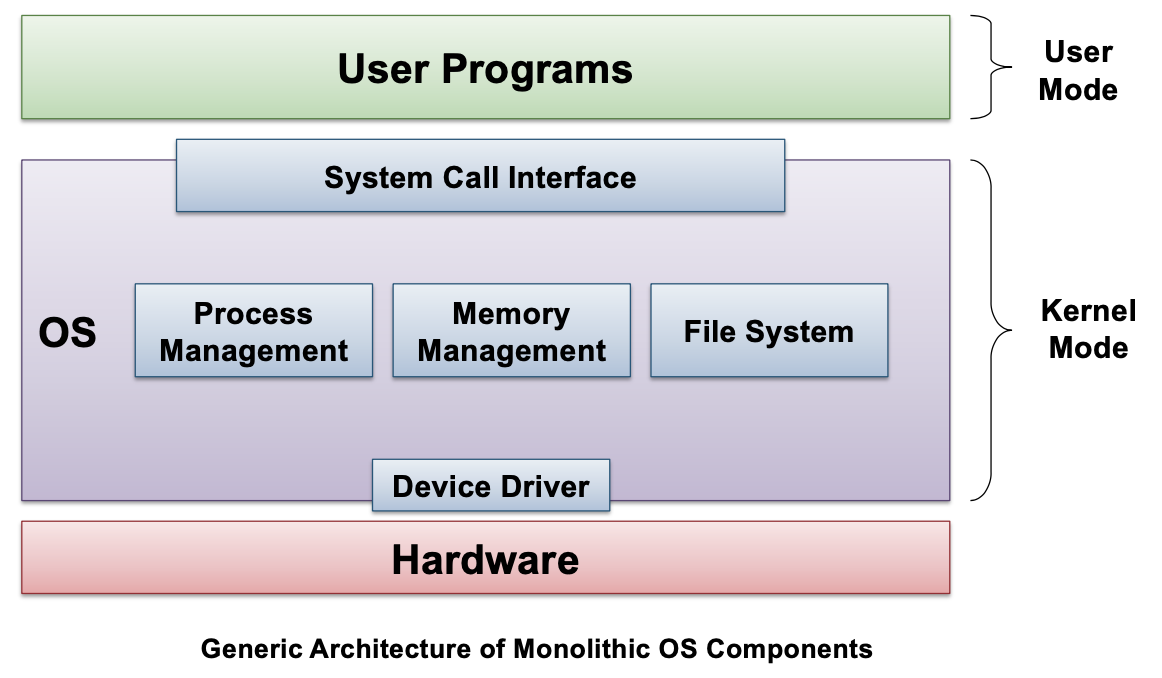
\includegraphics[scale=.4]{./assets/monolithicOs.png}

		\textbf{Microkernel OS}
		
		Kernel is \green{small and clean}, provides only essential and basic features like

		\tab - IPC, address space management, thread management, etc.

		Higher Level services run on top of basic facilities

		- runs as server process outside OS

		- uses IPC to communicate

		\green{Advantages}: Kernel more robust and extendible, better isolation and protection 
		between kernel and high level services

		\red{Disadvantages}: Lower performance

		% 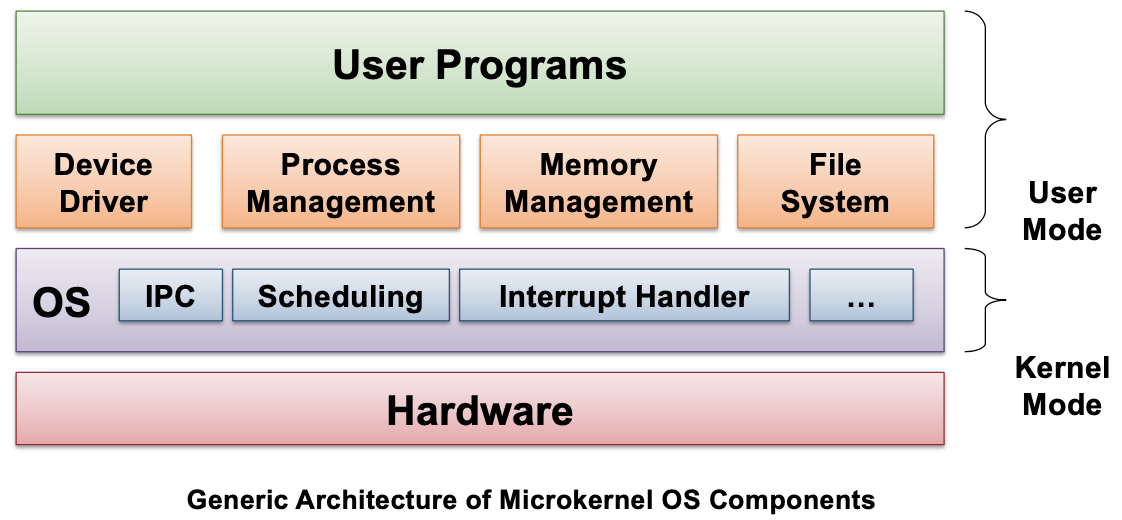
\includegraphics[scale=0.4]{./assets/microkernelOs.png}\\

		% \textbf{Virtual Machines aka Hypervisor}: To run multiple OS / debug and monitor OS

		% Definition: software emulation of hardware

		% - virtualisation of underlying hardware (illusion of complete hardware to level above)

		% Type 1 Hypervisor

		% - runs on hardware, can run multiple OS on it

		% - provides individual VM to guest OS

		% Type 2 Hypervisor

		% - runs on host OS

		% - Guest OS runs inside Virtual Machine

		\header{Process Abstraction}

		\textbf{Process}: abstraction over program information, allows multiple programs to share hardware

		OS representation of process includes \highlight{all information required} to describe running program

		1. Memory Context - code, data, stack, heap

		2. Hardware Context - registers, PC\dots

		3. OS Context - Process ID, Resources used\dots

		\textbf{Stack Memory}: Used for function invocation 
		
		Solves control flow and data storage issues, grows upwards

		Consists of:

		- return address of callee

		- parameters of function

		- storage of local variables

		- Frame Pointer: points to fixed location in stack frame (platform dependent)

		- saved registers

		\textbf{Stack Pointer}: Points to top of stack (first unused location)

		\textbf{Saved Registers}: limited registers in CPU, when exhausted

		\tab{} - use memory to temporarily hold the value

		\tab{} - Register can then be used by the funtion and restore after

		\tab{} - \highlight{register spilling}
		
		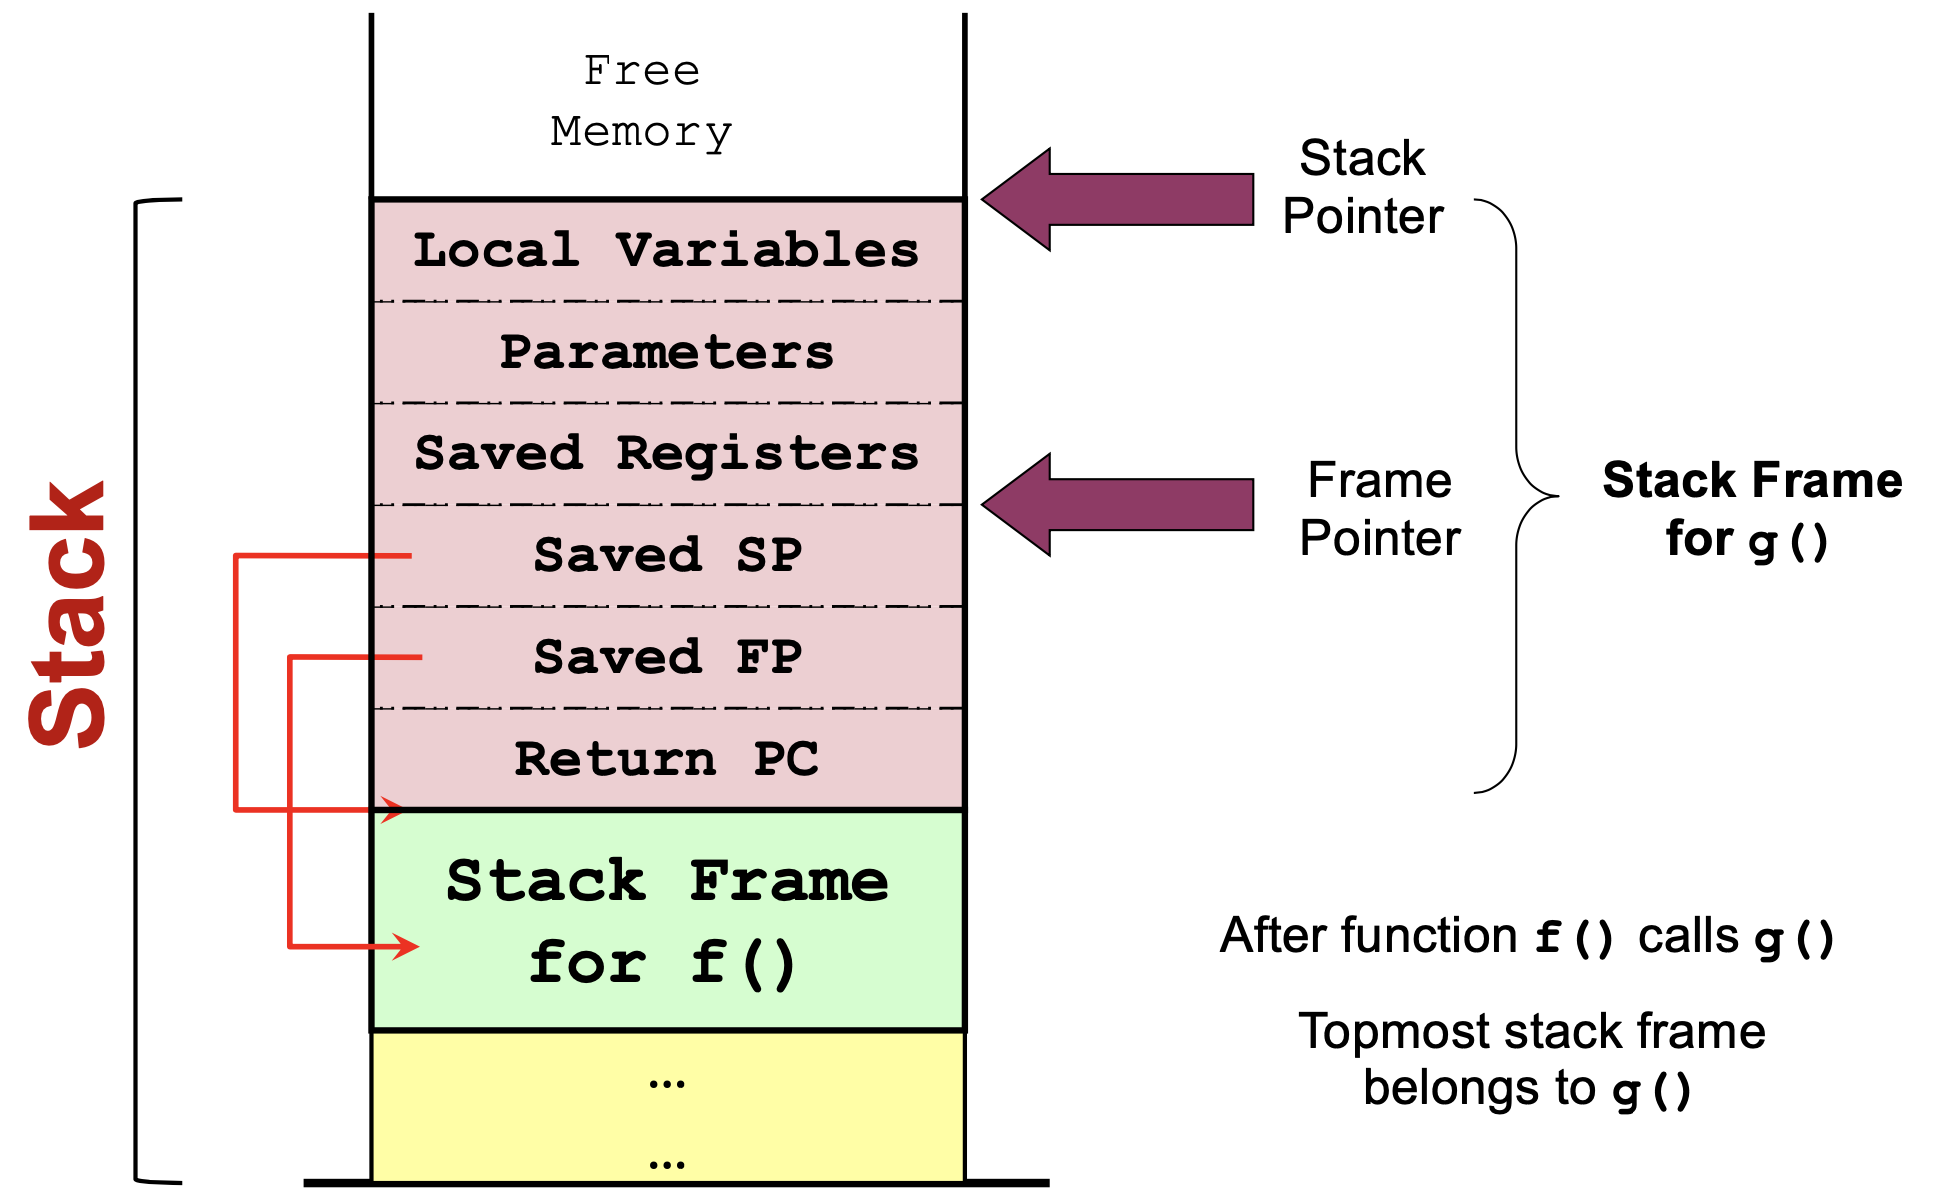
\includegraphics[scale=.2]{./assets/stackFrame.png}

		Call Convention: No universal way - hardware and PL dependent

		Setup:

		\red{Caller:} Pass parameters with registers / stack

		\red{Caller:} Save Return PC on stack

		\green{Callee:} Save registers used by callee, old FP, SP

		\green{Callee:} Allocate space for local variables of callee on stack

		\green{Callee:} Adjust SP to point to new stack top

		Teardown:

		\green{Callee:} Place return result on stack (is applicable)

		\green{Callee:} Restore saved registers, FP, SP

		\red{Caller:} Utilise return result if applicable

		\red{Caller:} Continues execution
		
		\textbf{Heap Memory}: For dynamically allocated memory $\rightarrow$ acquire memory at runtime

		Cannot use existing data / stack memory

		- size not known during compilation time (cannot Data)

		- no definite deallocation timing, accessible from anywhere (cannot Stack)

		Harder to manage: variable size, (de)allocation timing, can result in ``holes''

		\textbf{OS Context}

		PID - process ID, a number, unique among processes

		Process State - Indication of the execution status

		eg Generic 5-state process model

		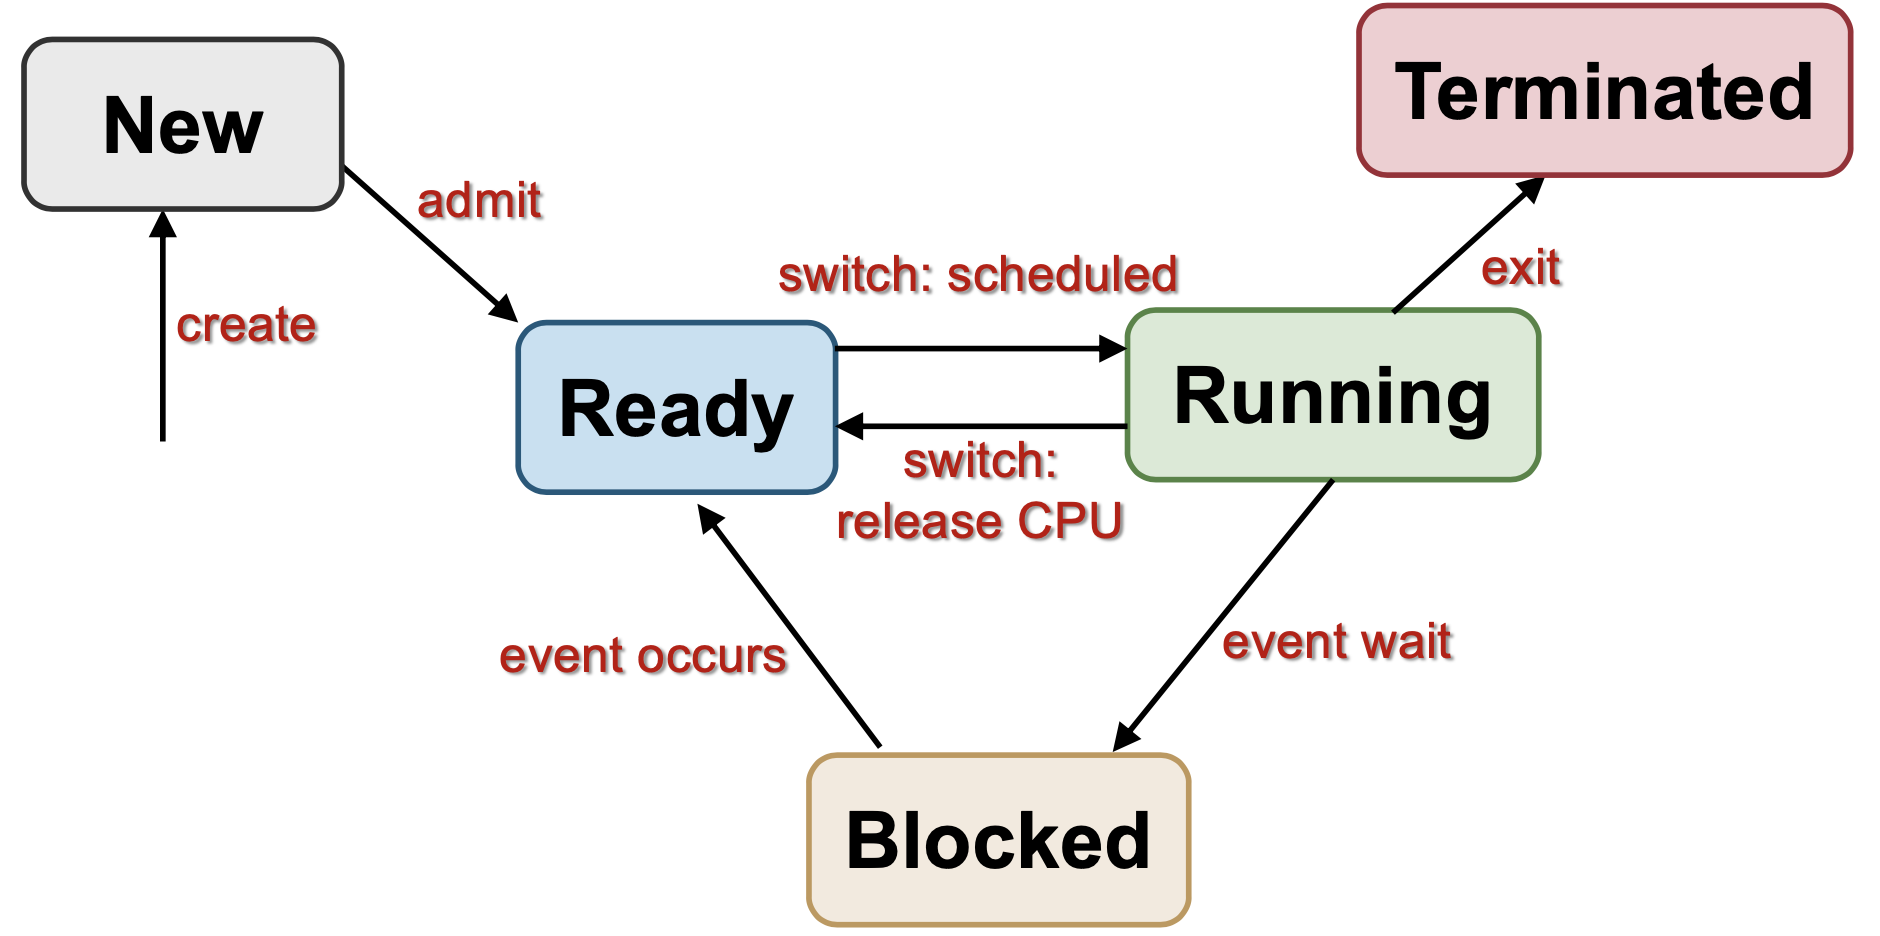
\includegraphics[scale=.2]{./assets/5ProcessState.png}

		New - just created, may be under initialisation (not ready to run)

		Blocked - waiting (sleeping) for event, cannot execute until event available

		Terminated - Process has finished execution, may require OS cleanup

		\textbf{Process Control Block and Table}

		Process Control Block: execution context of process (aka Process Table Entry)

		Kernel maintains PCB for all processes

		- in one table conceptually aka Process Table

		% 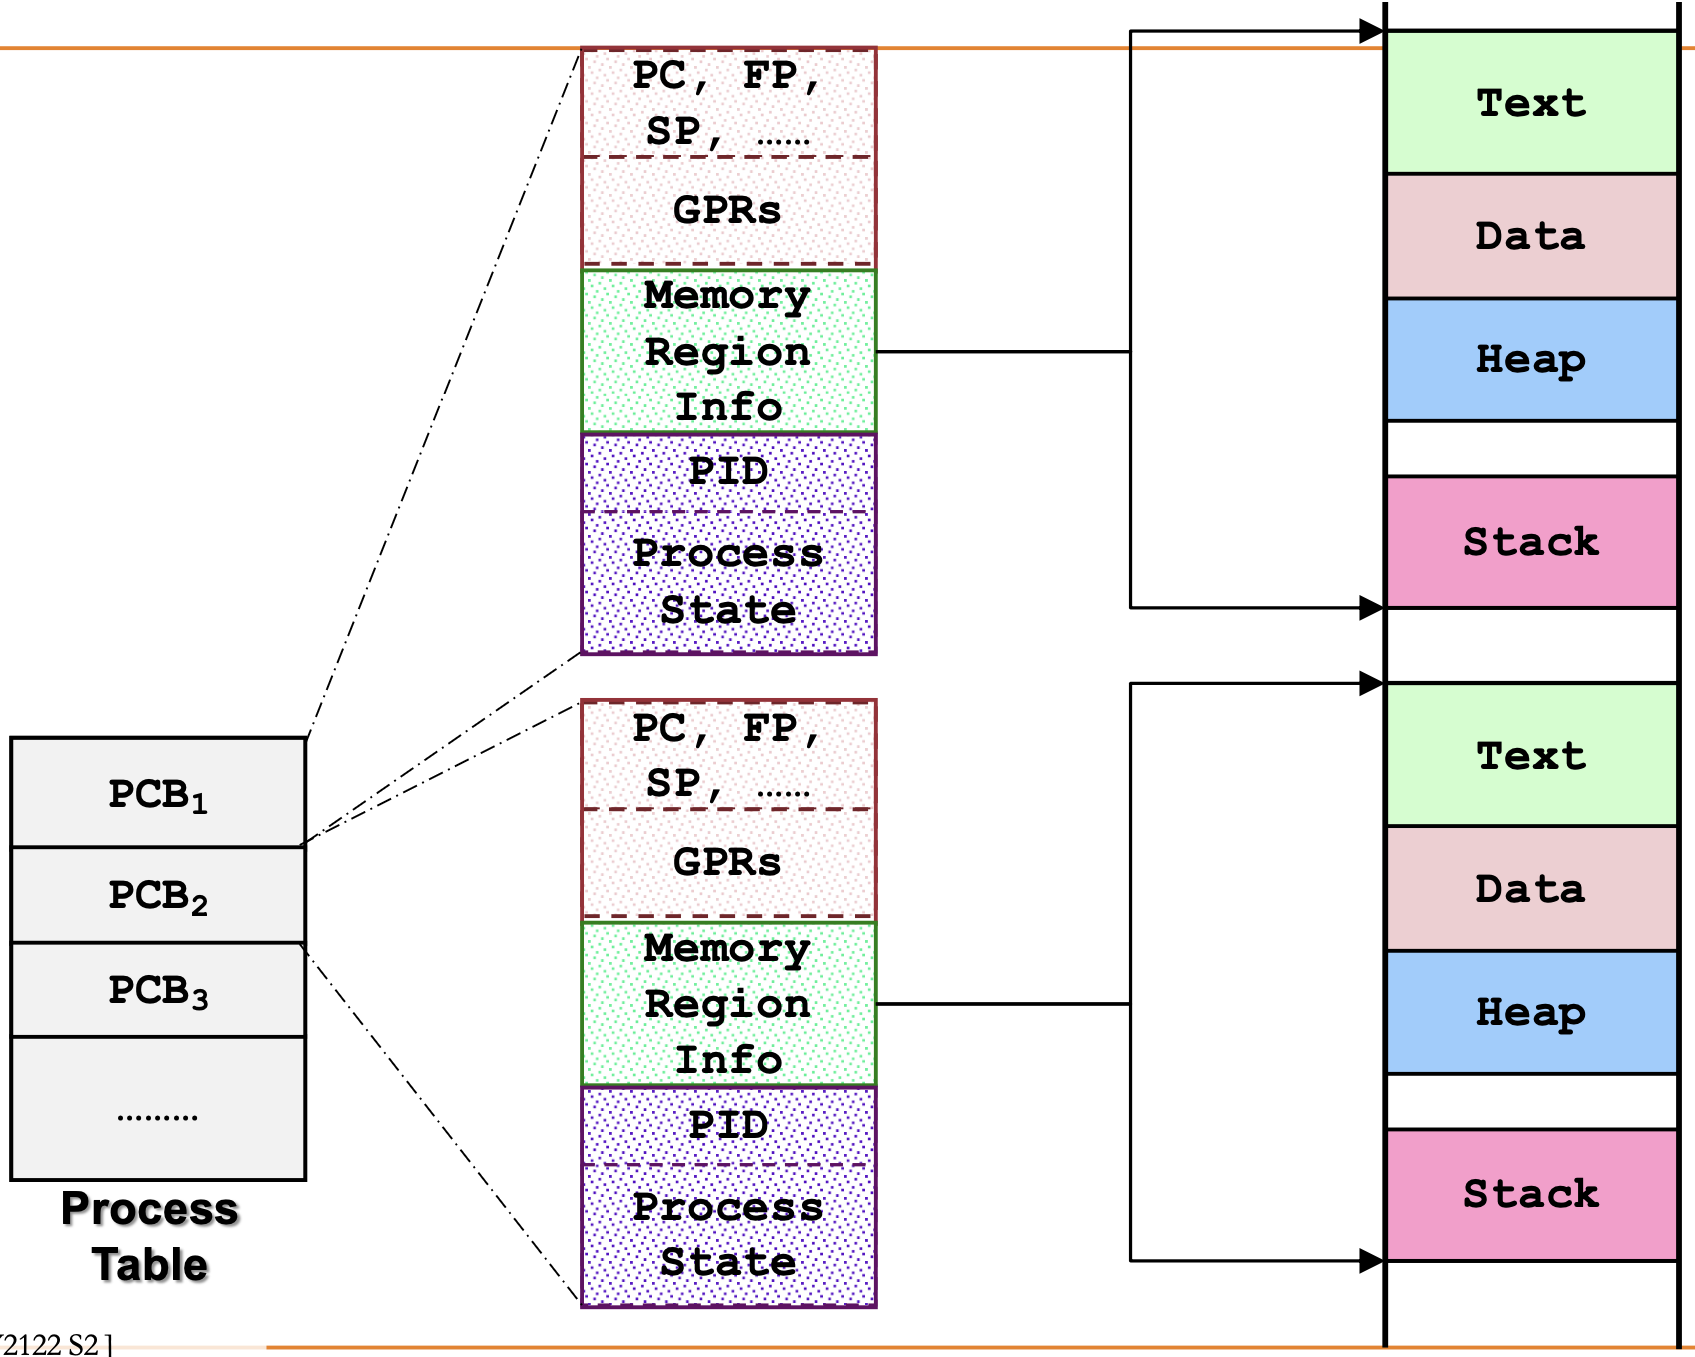
\includegraphics[scale=.2]{./assets/processTable.png}

		\textbf{Context Switch}

		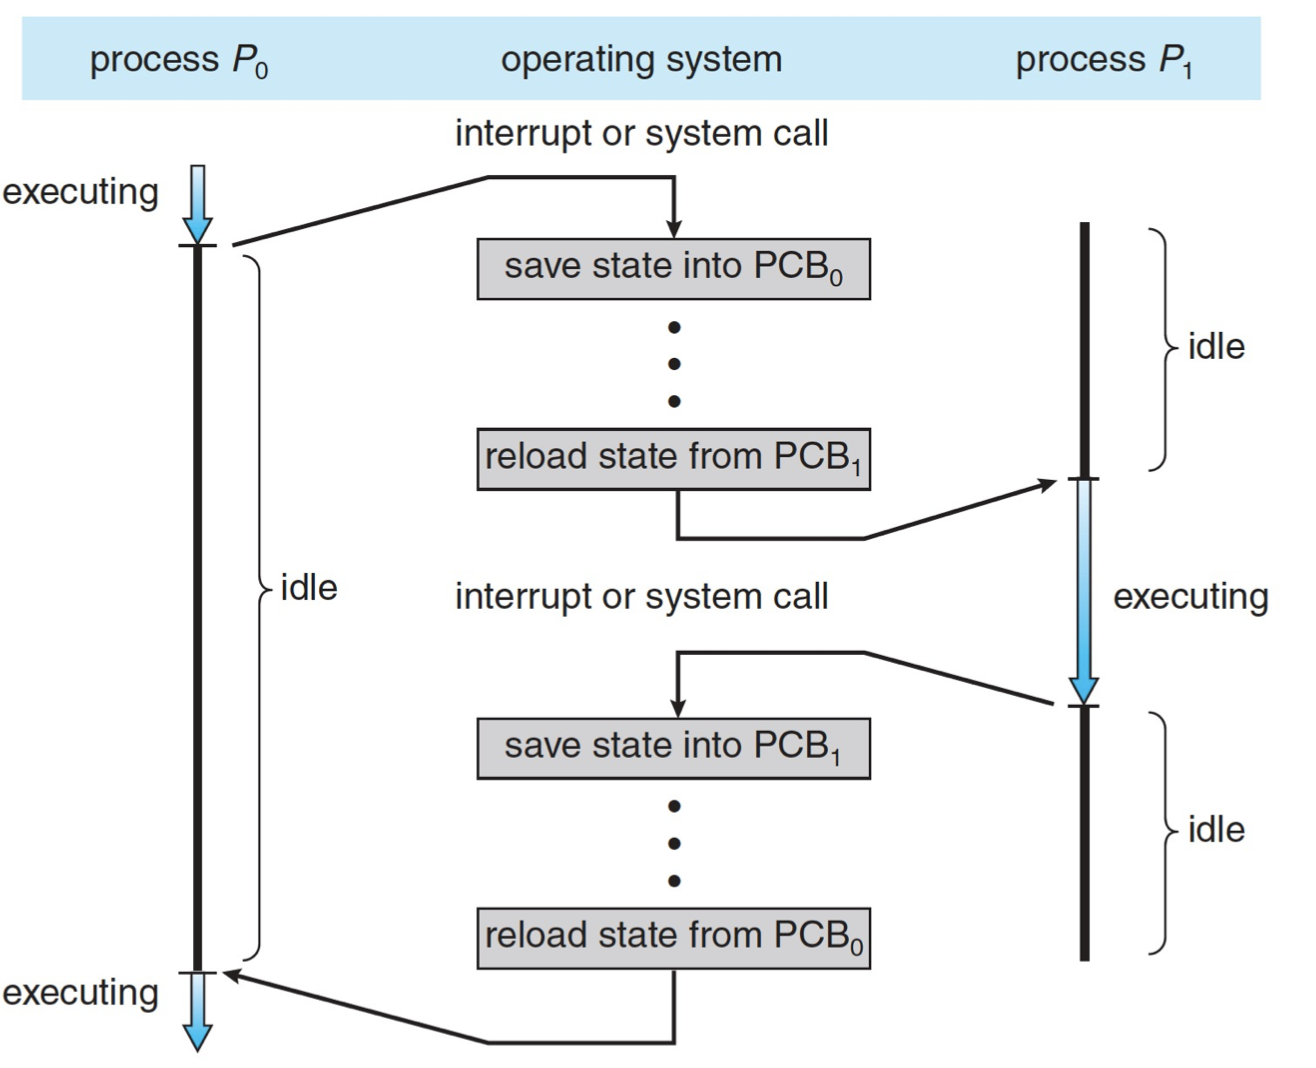
\includegraphics[scale=0.28]{./assets/contextSwitch.png}

		\textbf{System Calls}: API to OS, way to call services in kernel

		\highlight{NOT} a normal function call, need to change from \green{user} to \red{kernel} mode

		Call Mechanism

		1. User Program invokes library call

		2. Lib Call places \highlight{system call number} in a designated location

		\tab{} - eg. register (usually in assembly)

		3. Lib call does special instruction, switch from \green{user} to \red{kernel} mode

		\tab{} - known as \textbf{TRAP}

		4. In Kernel Mode, appropriate system call handler is determined

		\tab{} - Using the syscall number as index, handled by \textbf{dispatcher}

		5. Syscall handler is executed

		6. Handler finishes and returns control to lib call, switch back to \green{user} mode

		7. Lib call return to the user program, via normal function return mechanism

		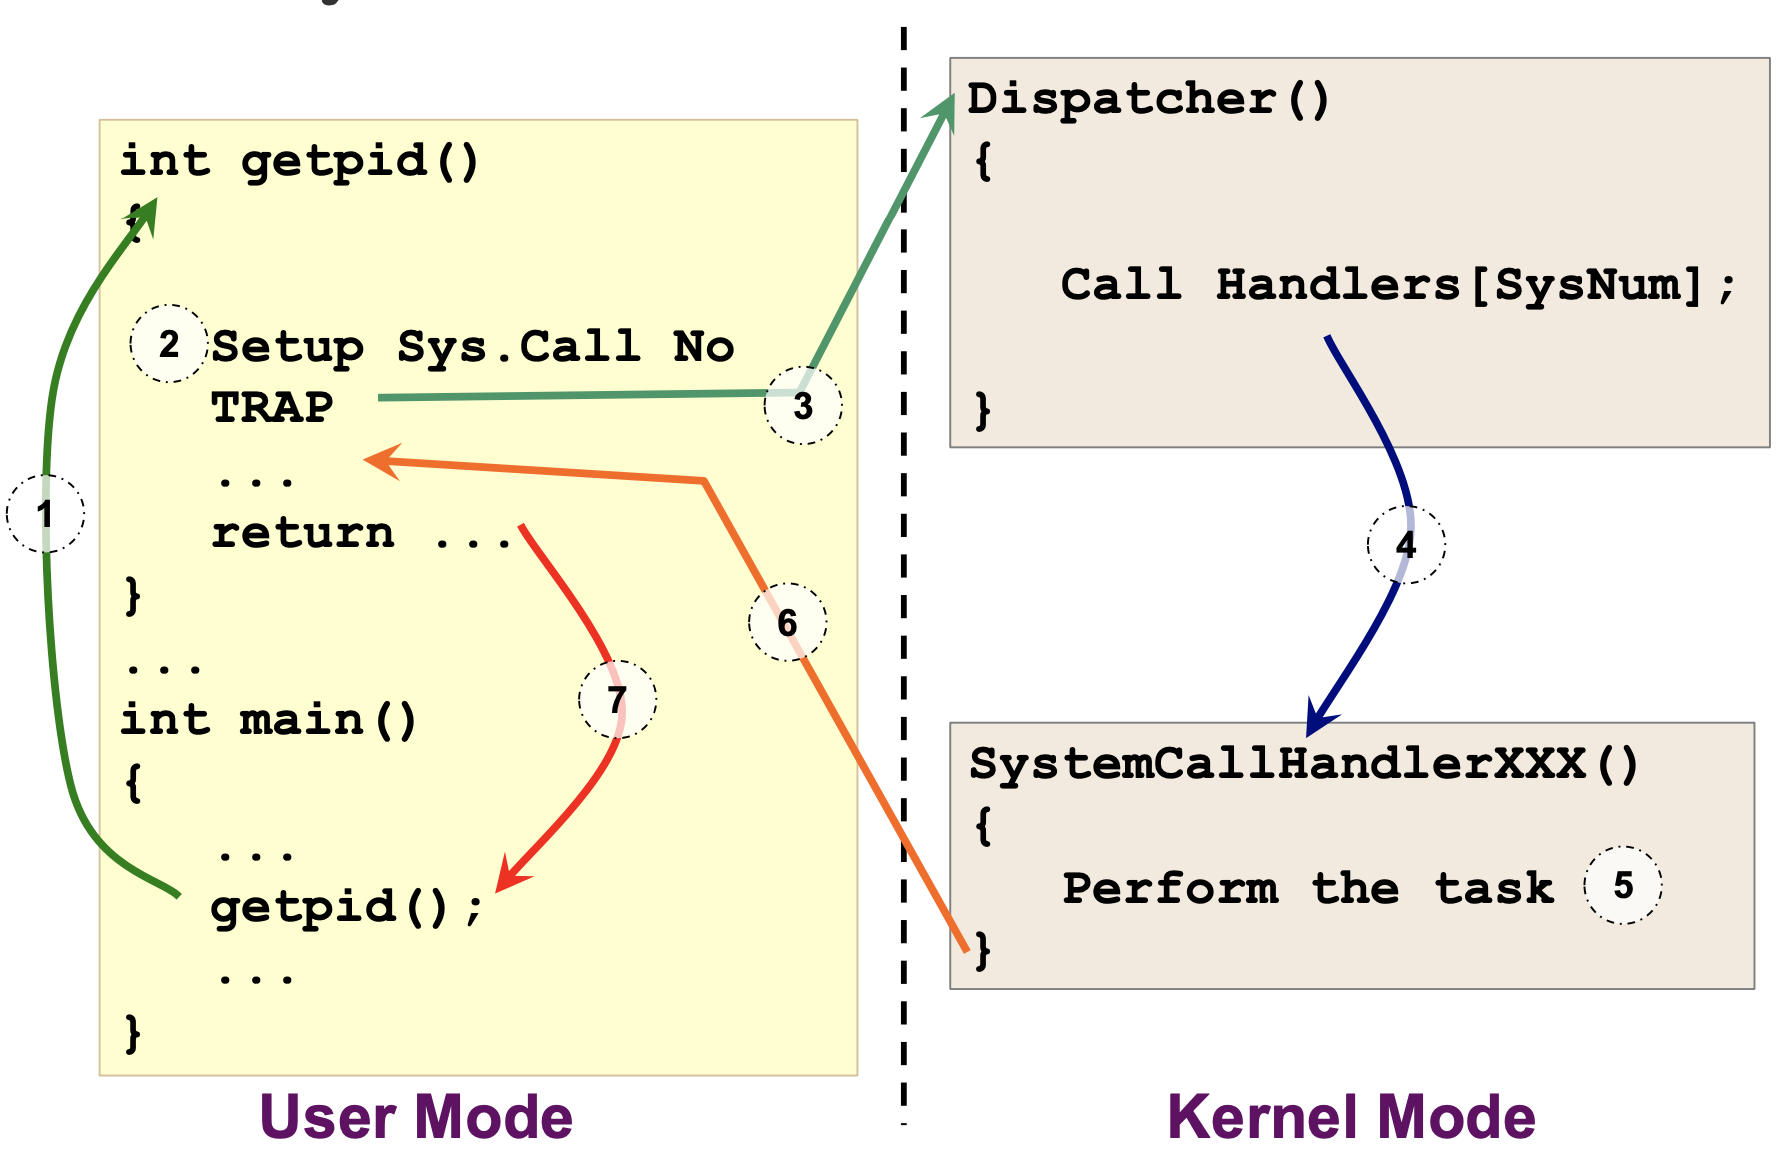
\includegraphics[scale=.24]{./assets/syscall.png}

		\textbf{Exceptions}: Happens when executing \textbf{machine level instruction}

		eg. Overflow, underflow, divide by 0, illegal or misaligned mem access

		Exception is \highlight{synchronous}

		\tab{} - occurs due to \red{program execution}
		
		Effect: Have to execute \highlight{Exception Handler}, like forced function call

		\textbf{Interrupt}: External events can interrupt execution of program

		Usually hardware related: timer, keyboard, mouse

		Interrupt is \red{asynchronous}, due to events \blue{independent} of program execution

		Effect: Program execution suspended, execute \textbf{interrupt handler}

		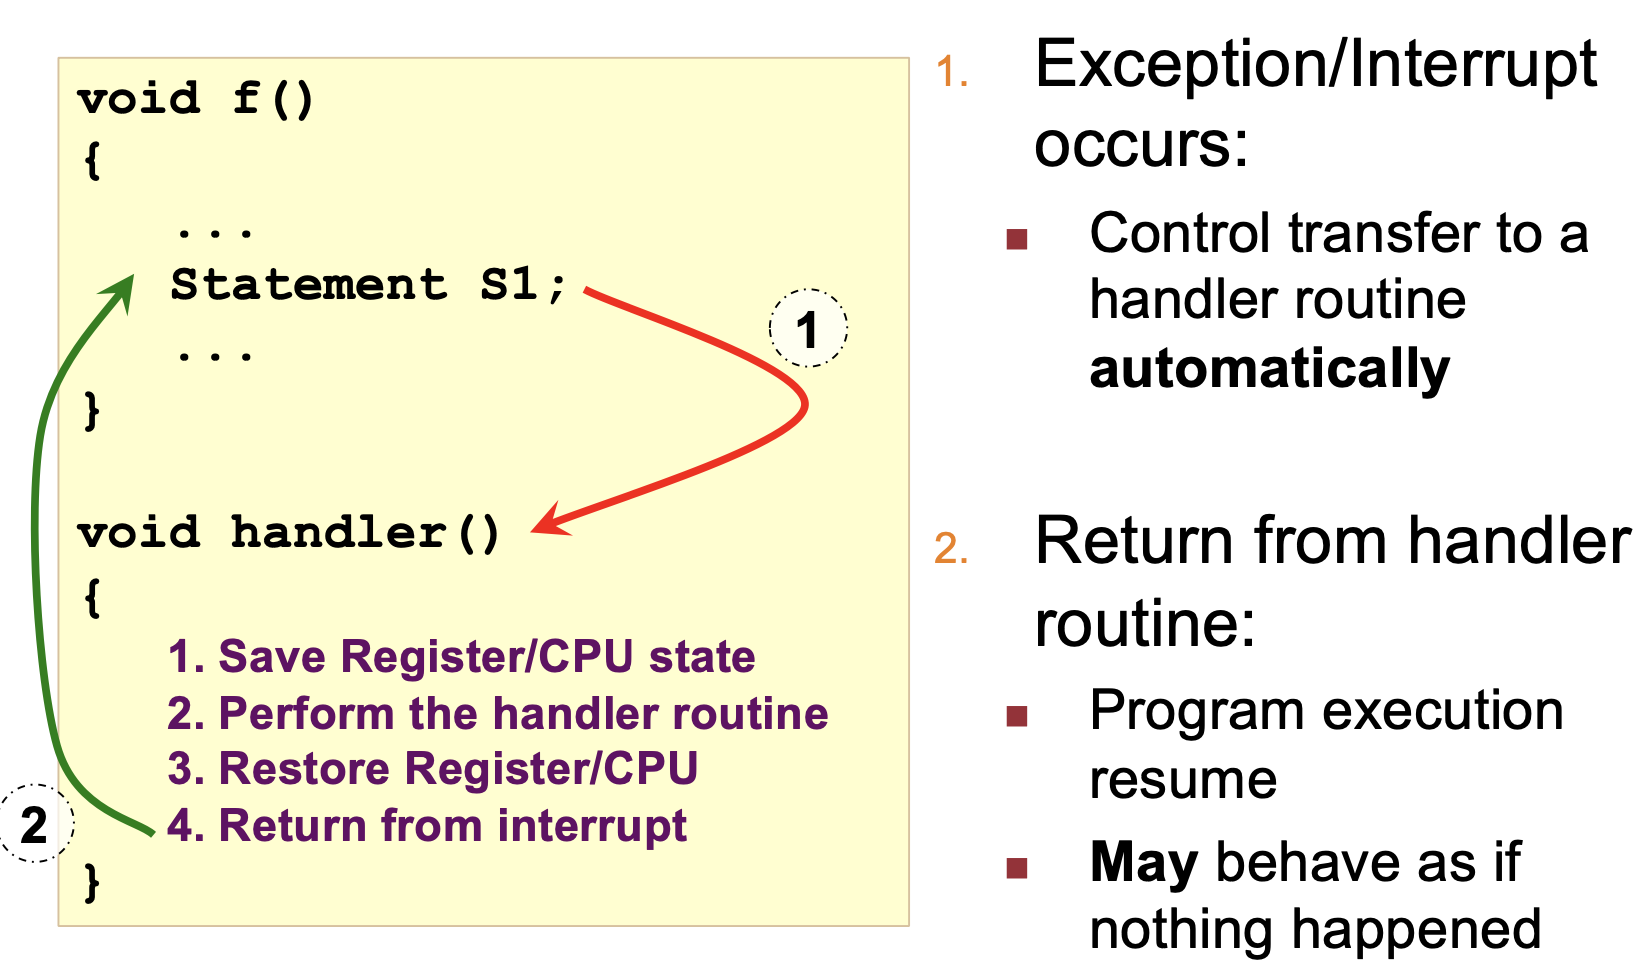
\includegraphics[scale=.25]{./assets/ExceptionInterrupt.png}

		\header{Process Abstraction in Unix}

		same as above just add \textbf{zombie} process state

		\textbf{Process Creation --- fork}

		syntax: \texttt{int fork()}

		Returns: \textbf{PID} of new process if \highlight{parent} 0 if \highlight{child}


		Behaviour: Creates child process that is a \textbf{duplicate} of current executable

		\tab{} - same code, same address space

		\tab{} - Data in child is a \highlight{COPY} of the parent (not shared)

		- \highlight{Differs in}: Process Id (PID), parent PID (PPID), \texttt{fork()} return value

		- Both parent and child continue executing after \texttt{fork()}

		- Use return value of \texttt{fork()} to distinguish between parent and child

		Implementation Optimisation: memory copy is very expensive

		- \green{Copy on Write}: If child only reads, or overwritten with \texttt{execl}, don't need to copy

		- duplicate a memory location when it is written to, o.w share memory

		\textbf{Execute new program --- execl}

		To replace current executing process image with new one

		Syntax: \texttt{int execl(const char *path, const char * arg0, \dots, const char *argN, NULL)}

		\tab{} - path: Location of executable

		\tab{} - arg0 - argN: command line arguments

		\tab{} - NULl: indicate end of argument list

		eg. \texttt{execl(``/bin/ls'', ``ls'', ``-l'', NULL)}

		\red{Note}: \highlight{Does NOT} return to program after completion of new image!

		\textbf{Process Termination in Unix --- exit}

		Ends execution of process

		Syntax: \texttt{void exit(int status)}

		\tab{} - status: returned to parent process, Unix convention: 0 okay, !0 not okay

		The function \highlight{does not return}

		Behaviour:

		- \textbf{Most} system resources used by process are released on exit, like FDs

		- Some resources not releasable

		\tab{} - PID and status (for parent-children sync), PCB \highlight{may} still be needed\\

		\textbf{Parent-Child Sync}: Parent process can wait for child process to terminate

		Syntax: \texttt{int wait(int *status)}

		Returns: PID of terminated child

		\tab{} - status (address): stores the exit status of terminated child process

		\tab{} - can use NULL if not needed

		Behaviour:

		- Blocking: blocks until \highlight{at least one} child terminates

		- Cleans up remainder of child system resources - kills zombie processes

		- Useful variants:

		\tab{} - waitpid(): waits for specific child process

		\tab{} - waitid(): waits for any child process to change status

		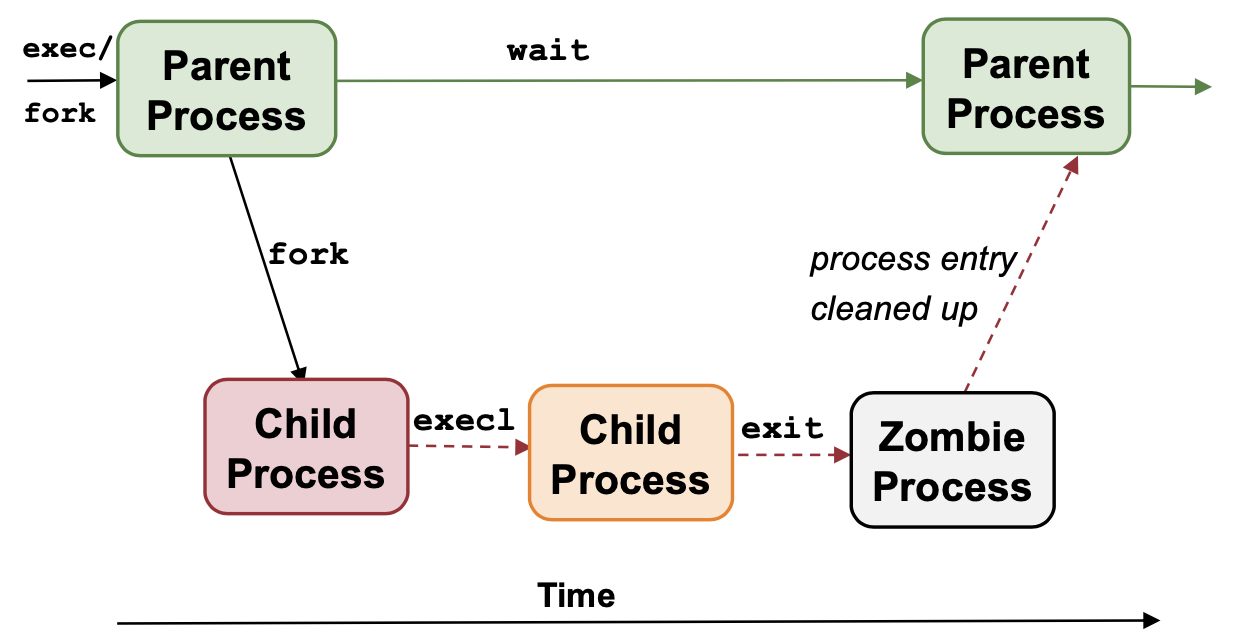
\includegraphics[scale=.3]{./assets/parentChild.png}

		\textbf{Zombie Processes}

		1. Parent terminates before child:

		\tab{} - \texttt{init} becomes pseudo parent of child

		\tab{} - child termination sends signal to \texttt{init}, which calls \texttt{wait} to cleanup

		2. Child process terminates before parent but parent did not call wait()

		\tab{} - Child process becomes zombie, can fill up process table

		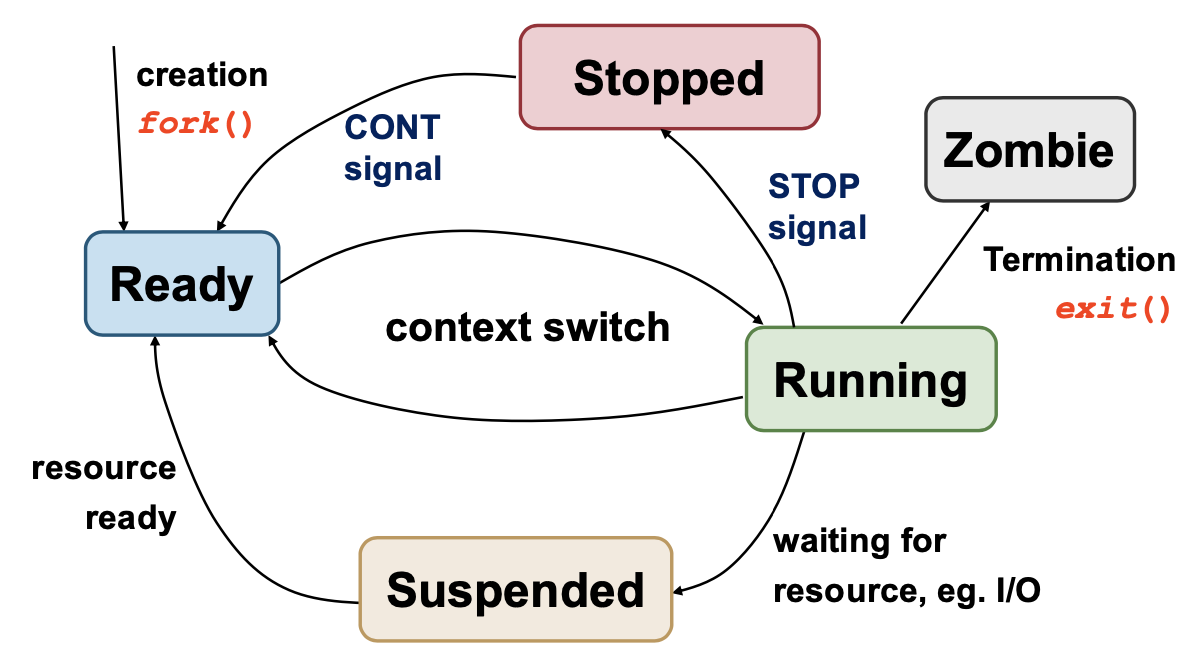
\includegraphics[scale=.3]{./assets/processStateUnix.png}

		\header{Process Scheduling}

		Concurrent execution: Both make progress within a short window of time
		
		\textbf{Processing Environment}

		1. Batch Processing

		\tab{} - long-running without user intervention $\rightarrow$ \highlight{no need} to be \blue{responsive}

		2. Interactive --- has active users interacting with it

		\tab{} - \highlight{responsive, consistent response time}
		
		3. Real time --- have a strict deadline to meet
		
		\textbf{Criteria for all scheduling algos}

		Fairness: no starvation, \textbf{per user} or \textbf{per process}

		Balanced Utilisation of System Resources

		- all components of the system should be utilised without bottlenecks

		\textbf{Preemptive vs Non-Preemptive}

		Non-preemptive: Process stays running until \blue{blocks} or \blue{yields CPU}

		Preemptive: CPU can be taken from running process at \green{any} time

		- process usually given a \red{time quantum} to run

		\tab{} - at end of \red{time quantum} process suspended (ready state)

		\tab{} - process can block / yield CPU early

		\textbf{Batch Processing Algos}: no user interaction
		
		- non-preemptive scheduler predominant (no need to be responsive)

		- Criteria:

		\tab{} - Throughput: rate of task completion

		\tab{} - Turnaround time: finish time - start time (time when process arrives)

		\tab{}\tab{} - related to \red{waiting time}: time spend waiting for CPU

		\tab{} - CPU Utilisation: \% of time when CPU is working

		1. \textbf{First Come First Served (FCFS)}: FIFO queue (based on arrival time)

		- blocked tasks are placed at back of queue

		- \highlight{no starvation}: no. of tasks in front are always decreasing

		Shortcomings:

		\tab{} - Convoy effect: short tasks stuck behind long task

		\tab{} - System resources sit idle

		2. \textbf{Shortest Job First}: Select task that needs the shortest amount of CPU time

		- Need to know \red{total CPU time} for a task in advance

		- minimises \highlight{average waiting time}

		- \highlight{Starvation possible}

		Guessing CPU time: guess future cpu time from previous cpu bound phases

		\tab{} - exponential average: $Predicted_{n+1} = \alpha Actual_n + (1 - \alpha)Predicted_n$

		3. \textbf{Shortest Remaining Time}: \highlight{preemptive} version of SJF

		- New jobs with shorter remaining time \highlight{can preempt} currently running job

		- good service for short job even if arrive late

		\textbf{Interactive environment}

		Criteria

		\tab{} - Response time: time between request and response

		\tab{} - predictability, less variation in response time better

		Timer 

		- Interval Timer Interrupt (ITI): OS scheduler is triggered every timer interrupt

		- Time Quantum: Execution duration given to process, constant / variable, multiple of ITI

		1. \textbf{Round Robin (RR)}: \red{preemptive version} of FCFS

		- Response time guaranteed, Timer needed

		- Choice of TQ:

		\tab{} big: CPU utilisation better, but longer wait time

		\tab{} small: more overhead $\rightarrow$ worse CPU utilisation, shorter waiting time

		2. \textbf{Priority Scheduling}: Tasks have priority, select tasks with $\uparrow$ priority

		- Preemptive: higher priority can preempt lower priority running process

		- Nonpreemptive: wait for next round of scheduling

		- can \highlight{starve lower priority}

		\tab{} - can decrease priority of running process after every round

		\tab{} - give each process minimum TQ

		3. \textbf{Multi-Level Feedback Queue}: \green{Adaptive} --- Learns process behaviour 

		- Tries to minimise response time for interactive and IO bound process and

		- Turnaround time for CPU-bound processes

		Rules

		- if priority(A) > priority(B), then B, if equal, RR

		- New job: \green(highest priority)

		- job fully utilises its TQ: \red{priority reduced}

		- job blocks / yields CPU before TQ: \green{priority retained}

		4. \textbf{Lottery Scheduling}: Scheduling done in rounds, with lottery tickets

		in each round:

		\tab{} - give out lottery tickets for resources

		\tab{} - When scheduling decision, choose \red{random ticket w/o replacement}

		- In every round, process w \blue{X\%} of tickets gets to use resource \blue{X\%} of time

		- \red{Responsive}: Every participating process gets to run every round, new processes can participate in next round

		- \red{Good control}: important process given more tickets\\

		\header{Inter-Process Communication}

		\textbf{Race Condition}

		If multiple accesses to a shared variable while modifying
		
		\textbf{Shared Memory}: Communication through read/write to shared variables

		1. $P_1$ creates shared memory region $M$

		2. $P_2$ attaches $M$ to its own memory space

		3. $P_1$ and $P_2$ can communicate through $M$

		\green{Advantages:}

		- Efficient: OS only needed in setup, Easy to use: just like normal memory

		\red{Disadvantages:}

		- Limited to one machine, Requires synchronisation because of data races

		\textbf{Message Passing}: \red{Explicit} communication through exchange of messages

		- $P_1$ prepares message $M$ and send to $P_2$

		- $P_2$ receives message $M$

		- sending and receiving provided as syscalls

		Naming Scheme: how to identify other party (parties)

		Synchronisation: blocking/ non-blocking

		Naming Scheme: \textbf{Direct Communication}: \red{Explicitly name} other party

		- One link per pair of communicating processes

		- Need to know the identity of the other party

		Naming Scheme: \textbf{Indirect Communication}: Messages sent to mailbox

		- one mailbox shared among many processes

		Blocking (\textbf{Synchronous}):

		\texttt{send()}: sender is blocked until message received

		\tab{} - does not require buffer, sender can keep until receiver calls \texttt{receive}

		\texttt{receive()}: blocked until message arrived

		Non-blocking (\textbf{Asynchronous}):

		\texttt{send()}: sender resumes immediately

		\tab{} - never blocked unless buffer full (can throw error also)

		\tab{} - finite buffer means not truly async

		\texttt{receive()}: message hasn't arrived then just continue

		\textbf{Message Buffer}

		- OS control: no synchronisation necessary

		- decouples sender and receiver, no need to unnecessarily wait

		\green{Advantages:}

		- applicable beyond one machine

		- Portable: parties on different platforms can communicate

		- Easier synchronisation

		\red{Disadvantages:}

		- Inefficient: requires OS intervention on every send and receive

		- Harder to use: must use specific data format

		\textbf{Pipes}

		Process has 3 communication channels: \texttt{stdin, stdout, stderr}

		Shell uses ``|'' symbol to link input output channels from one process to another

		General Idea: Communication channel has 2 ends --- read and write

		- writers \red{wait} when buffer is \red{full}

		- readers \red{wait} when buffer is \red{empty}

		Syntax: \texttt{int pipe(int fd[])}

		Returns: 0 for success, !0 for failure

		fd[0] == reading end, fd[1] == writing end

		\textbf{Signal}: Asynchronous notification

		Recipient must handle by: \blue{default handlers} or \blue{User supplied handlers}\\

		\header{Threads - lightweight process}

		cheaper alternative to processes (fork is expensive)

		- duplicate memory space, most of process context

		- context switch requires saving/restoring process info

		Communication difficult and inefficient (independent memory space)

		- requires IPC

		Multiple threads = multiple parts of progran executing concurrently

		\textbf{Threads}

		Threads share:

		- \textbf{Memory context:} Text, Data, Heap \highlight{NOT stack}

		- \textbf{OS Context:} PID, other resources like files

		Unique info: thread ID, stack, registers (hw context)

		\textbf{Thread Switch vs Context Switch}

		\red{Context switch} involves: Memory, OS, Hardware context

		\green{Thread switch} involves: Hardware Context, Stack (change FP and SP)

		\green{Benefits}

		- Economy: require much less resources to manage compared to processes

		- Resource Sharing: share most resources of process, no need for IPC 

		- Responsiveness: can appear much more responsive

		- Scalability: take advantage of multiple cores/CPU

		\red{Problems}

		- Synchronisation around shared memory harder

		- System Call concurrency: OS must guarantee correctness and determine correct behaviour

		- Process Behaviour: \texttt{fork()} duplicates threads? \texttt{exec()} changes all threads?

		\textbf{Thread Models}

		1. \textbf{User threads}: implemented as user lib

		- runtime system handles thread-related operations

		- Kernel is \highlight{not aware} of the threads within the process

		\tab{} - thread level scheduling \red{not possible}

		\green{Advantages}

		- Can have multithreaded program on \textbf{any OS}

		- Thread operations are just library calls

		- More flexible and configurable (user-customised thread scheduling)

		\red{Disadvantages}

		- OS not aware of threads, scheduling performed at process level

		\tab{} - One thread blocked $\rightarrow$ process blocked $\rightarrow$ all threads blocked

		\tab{} - Cannot exploit multiple CPUs

		2. \textbf{Kernel Threads}: implemented in OS, thread operations are \red{syscalls}

		- Thread-level scheduling \green{is possible}, kernel schedules threads, not processes

		\green{Advantages}: Kernel can schedule on thread levels

		\red{Disadvantages}

		- Thread operations are now system calls

		\tab{} - slower and resource intensive

		- less flexible

		\tab{} - Used by all multithreaded programs

		\tab{} - implemented with many features $\rightarrow$ overkill for simple program

		\tab{} - implemented with few features $\rightarrow$ not flexible enough for some programs

		3. \textbf{Hybrid Thread Model}: Have both Kernel and User threads

		- OS schedules \highlight{kernel threads}

		- \green{User threads} can bind to \red{kernel threads}\\

		\header{Synchronisation}

		\textbf{Properties of Correct CS Implementation}

		1. Mutual Exclusion: at most 1 process in Critical Section

		2. Progress: if no process in CS, one of the waiting processes can enter

		3. Bounded Wait: Upper bound on no. of times others can enter before $P_i$

		4. Independence: Process \highlight{not} executing in CS should never block others

		\textbf{Symptoms of Incorrect Synchronisation}
		
		1. Incorrect output/behaviour: due to lack of mutual exclusion

		2. Deadlock: all processes blocked: no progress

		3. Livelock: processes keep changing state (avoid deadlock), but no progress

		4. Starvation: some processes blocked forever

		\textbf{HLL Implementation: Peterson's Algorithm}

		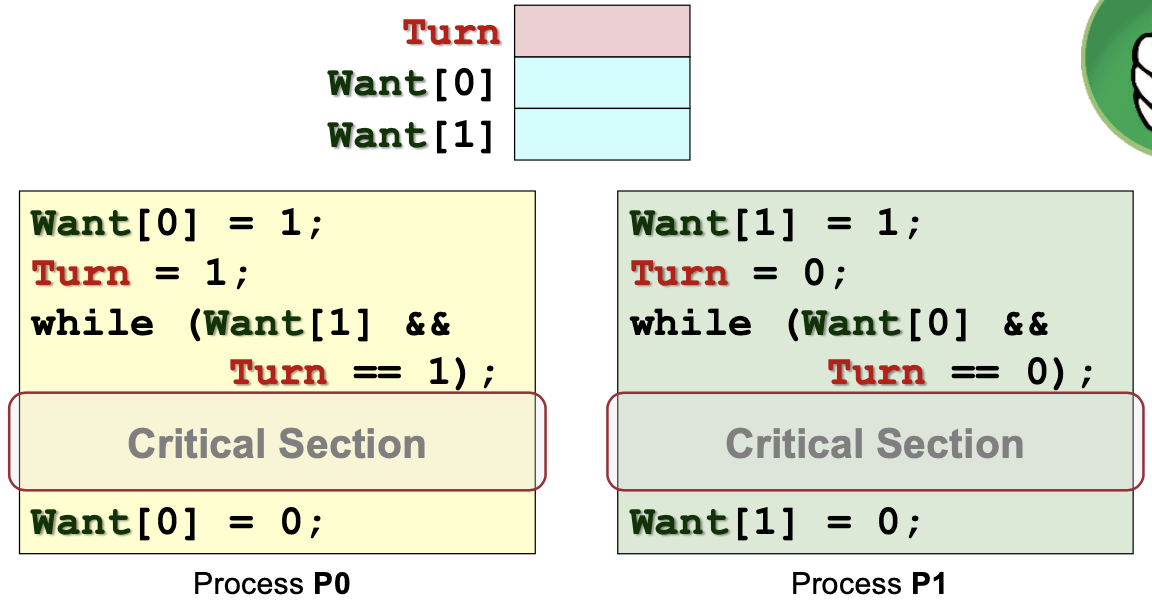
\includegraphics[scale=.3]{./assets/peterson.png}

		\red{Disadvantages:}

		1. Busy Waiting: keep testing while-loop (should block)

		2. Low Level and Not general: general synchronisation mechanism desirable

		\tab{} - not just mutual exclusion

		\textbf{Assembly Implementation: Test and Set}: Used to implement a \highlight{lock}

		syntax: \texttt{TestAndSet Register, MemoryLocation}
		
		Behaviour (\highlight{SINGLE ATOMIC machine operation}):

		1. Load current content at \texttt{MemoryLocation} into \texttt{Register}

		2. Stores \highlight{1} into \texttt{MemoryLocation}

		Note: Does \red{not} guarantee bounded wait out unless scheduling is fair

		Usage:
		\begin{verbatim}
		void EnterCS(int *lock) {
			while (TestAndSet(lock) == 1);
		}
		void ExitCS(int *lock) {
			*lock = 0;
		}
		\end{verbatim}

		\textbf{High Level Synchronisation Mechanism: Semaphore}

		- Only functional behaviour specified (can have different implementations)

		- Provides means to

		\tab{} - \highlight{block} a number of processes, known as sleeping processes (wait)

		\tab{} - unblock \ wake one or more sleeping processes (signal)

		\red{Note}: Both of these operations are \highlight{atomic}

		Semaphore contains an integer value, initialised to any non-negative value

		Invariant \red{always} holds: $S_{current} = S_{initial} + \#signal(S) - \#wait(S)$

		General/Counting Sem: S $\geq 0$, can be implemented with binary sempahore

		Binary Semaphore: S = 0 or 1
		
		\texttt{Wait(S)}: if $S \leq 0$: block, else: \textbf{Decrement} S

		- aka \texttt{P(), Down()}

		\texttt{Signal(S)}: \textbf{Increment} S, Wakes up sleeping process if any

		- \highlight{never} blocks

		- aka \texttt{V(), Up()}

		\highlight{Note:} Deadlock can occur with incorrect use of semaphore

		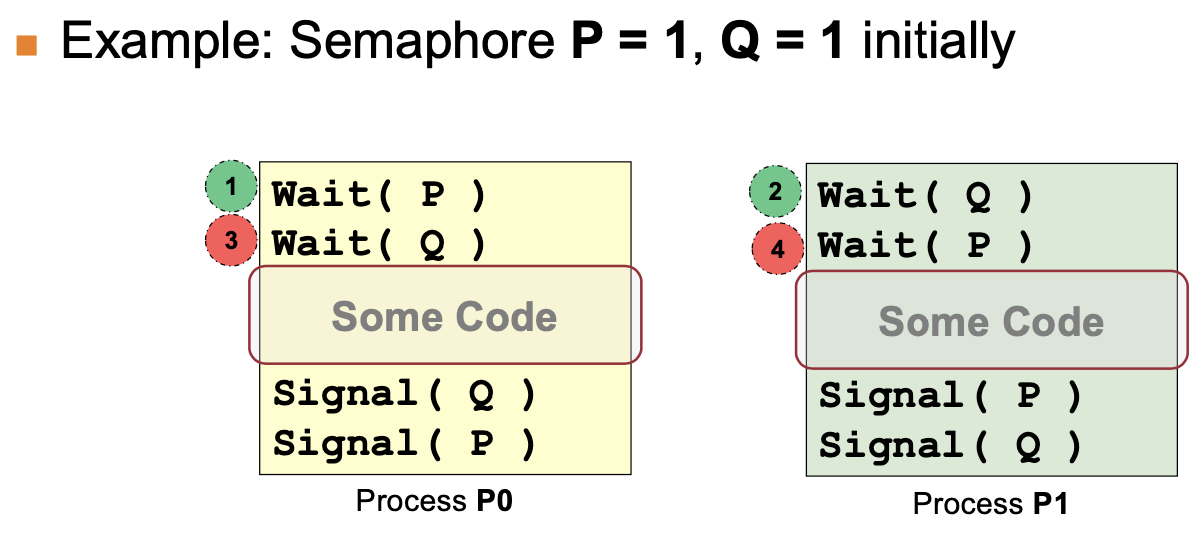
\includegraphics[scale=0.25]{./assets/semaphore-wrong.png}

		\header{Memory Management}

		OS \blue{allocates}, \green{manages}, \red{protects} mem space of process (from other processes)

		OS provides memory-related \red{syscalls} to processes

		\textbf{Memory Abstraction}

		1. \textbf{No Memory Abstraction}

		% \green{Pros}: address in program = physical address, \highlight{no conversion}, address fixed at compile time

		\red{Cons}: Processes cannot occupy same physical location (both start at 0)

		2. \textbf{Address Relocation (No HW support)}

		\red{Cons}: slow load time, hard to distinguish memory ref from normal int constant

		3. \textbf{Base and Limit Register (HW support)}

		% Special register as \red{base} (starting addr of process) of all memory references, and another as \green{limit}.

		% During compile time, all mem ref are compiled as offset from \red{base}, and accesses checked against
		% \green{limit} to protect mem space

		\red{Cons}: every access incurs addition and comparison

		% \textbf{Logical Address}: How the proces views its memory space

		% Logical addr != Physical addr: mapping between the two needed

		% Each process has self-contained, indep logical mem space

		\textbf{Contiguous Memory Management}

		Assumptions: Process occupies \red{contiguous mem region} and physical mem is large enough to contain process

		\textbf{Fixed Partitioning}: Process is given a fixed sized chunk of memory

		\green{Pros}: Easy to manage, fast to allocate (no need choose)

		\red{Cons}: Partition big enough for largest process, \highlight{internal fragmentation}

		\textbf{Dynamic Partitioning}: Process given exact amount of memory required

		\green{Pros:} Flexible and removes internal fragmentation

		\red{Cons}: maintain more info, longer to allocate (must choose), external fragmentation

		\textbf{Dynamic Partitioning Allocation Algos}

		OS maintains a list of partitions and holes

		1. \textbf{First-fit}: first hole that is large enough

		2. \textbf{Best-fit}: find the smallest hole that is large enough

		3. \textbf{Worst-fit}: find largest hole

		When partition freed, \highlight{merge} with adjacent holes if can

		Compaction: \red{Move occupied partitions} to create \green{bigger holes}, \highlight{costly}

		\textbf{Multiple Free Lists}

		1. Separate list of free holes from list of occupied partitions

		2. Keep multiple lists of diff hole sizes

		- Take hole from list that most closely matches request size

		- Partition size typically increases exponentially

		- Faster allocation

		\includegraphics*[scale=0.3]{./assets/multipleFreeList.png}

		\textbf{Buddy System}

		Provides efficient partition splitting, (de)allocation time and coalescing

		1. Free block split into half until meet request size

		\tab{} 1.1 two halves form buddy blocks

		2. When both buddies are free

		\tab{} 2.1 merge together to form larger block

		\includegraphics*[scale=.25]{./assets/buddy}

		\underline{Implementation}

		1. Keep array \texttt{A[0...k]} where $2^k$ is largest allocable block size

		\tab{} 1.1 each array element is LL keeping track of free blocks of that size

		\tab{} 1.2 Each free block is indicated just by starting address

		May have smallest allocable block size as well 

		\underline{Allocate Algo}: allocate block of size $N$

		1. Find smallest $S$ st $2^S \geq N$ 

		2. Access \texttt{A[S]}

		\tab{} 2.1 if exists: remove block, allocate block

		\tab{} 2.2 else:

		\tab{}\tab{} 2.2.1 Find smallest $R$ from $S + 1$ to $K$ that has free block

		\tab{}\tab{} 2.2.2 For ($R-1$ to $S$): repeatedly split till $S$, then go to 2

		\underline{Deallocate Algo}: free block B of size $2^S$

		1. Check \texttt{A[S]}, if buddy of B exists (free)

		2. If so, remove B and buddy from list, merge to get larger B'

		\tab{} 2.2 goto step 1, with B' as B

		3. else: insert B into \texttt{A[S]}

		Using \red{Binary}: blocks B and C are buddies if 

		1. Lowest $S$ bits (0 to $S$) are identical \red{and} Bit $S$ ($S + 1$ bit) is different\\
		
		\header{Disjoint Memory Schemes}

		Remove assumption that process occupies one contiguous memory block

		\textbf{Paging}: Memory split into \red{physical frames}

		Logical memory of process also split into \red{logical pages}, \green{same size}

		At execution time, pages are loaded into \highlight{any avail} frame

		\textbf{Lookup Mechanism}: Page Table

		Physical Address $=$ Frame Number  $\times$ sizeof(frame) $+$ offset

		Frame Number $=$ (Page\_Table [page\_no])

		Offset: displacement from beginning of physical frame

		\red{Note}: Keep frame size as power of 2, can use bit manipulation

		\textbf{Address Translation Formula}: frame size $2^n$, $m$ bit logical address

		1. Split LA into \red{$p = (m - n)$ MSB of LA} and \green{$o = $ remaining $n$ bits}

		2. Use $p$ to find frame number $f$ (from Page Table)

		3. $PA = f*2^n + o$

		\textbf{Properties}

		1. \green{No external fragmentation} as every single frame can be used

		2. \green{Insignificant internal fragmentation} - max 1 page per process not utilised

		3. Clean separation of LA and PA

		\textbf{Implementation}

		\red{Software solution}: OS stores PT info in PCB (part of mem context), pointer cos PT big

		\tab Issues: \red{2 mem accesses} per mem ref. 1st for PT, 2nd for memory item

		\green{Hardware Support}: Translation Look-Aside Buffer (TLB)

		- cache for PT entries, very small (10s of entries) fast ($\leq$ 1 clock)

		\textbf{Avg Access Time w TLB}: TLB 1ns, Memory 10ns, avg hit rate 90\%

		90\%(1ns $+$ 50ns) + 10\%(1ns $+$ 50ns $+$ 50ns) = 56ns

		\textbf{TLB and Context Switching}: TLB flushed

		Flushed for correctness, security, safety

		TLB is per core, must be fast so can't be centralised, part of pipeline (checked before access memory)

		\highlight{Note}: TLB is \red{not} part of hw context
		
		\textbf{Paging Protection}

		1. Access-Right Bit: Each PTE has (read, write execute) bits

		2. Valid bits: prevents mem access to unused pages 

		\highlight{Every} mem access checked against these bits \red{in hw}

		\textbf{Page Sharing}: Same frame number in PTEs of diff processes

		1. Share code page, eg. library code, syscalls

		2. Implement \highlight{Copy-on-Write}\\

		\textbf{Segmentation}

		Reasons:

		1. Split memory space according to \red{logical memory regions}

		\tab{} 1.1 diff regions have diff usages, permissions, lifetimes, etc

		2. Some regions may \green{grow} / \red{shrink} at execution time

		Each memory segment has a \red{name}, \green{limit}

		Memory References: \red{Segment name} $+$ \green{offset}

		\textbf{Logical Address Translation}

		Each segment maps to \red{contiguous} memory region with \red{base addr} and \green{limit}

		Logical Address $<$\green{SegId}, \blue{Offset}$>$

		1. SegId used to look up $<$Base, Limit$>$ of segment in \highlight{segment table}

		2. Physical Address $PA = Base + Offset$

		\red{Note}: Offset $<$ Limit for valid access

		\textbf{\green{Pros}}

		1. Each segment is indep contiguous memory space

		\tab{} 1.1 More efficient bookkeeping

		\tab{} 1.2 Segments can grow / shrink and be protected / shared independently

		\highlight{Cons}

		1. Requires \red{variable-size contiguous} memory region 
		
		\tab{} 1.1 external fragmentation

		\textbf{Segmentation with Paging}

		Segment composed of several pages instead of contiguous mem region

		\tab{} - Each segment has a PT 

		Segment can allocate new page and add to its PT to grow, and shrinks similarly

		\includegraphics*[scale=0.27]{./assets/segmentationPaging}

		Memory ref: \red{SegId}, \green{Frame no}, offset OR \red{SegId}, \green{offset}

		\tab{} - calculate frame number from offset in the second case\\

		\header{Virtual Memory Management}

		Remove second assumption that process can fit in memory

		\textbf{Idea}: Split logical addr space into chunks, some in memory, others in \red{secondary storage}

		Extension of paging: some pages in memory, some in secondary storage

		\textbf{Extended Paging Scheme}

		Still uses PT for Logical to Physical address translation

		Page Types: Mem resident vs non-mem resident (need new \red{resident} bit)

		\red{Page Fault}: CPU tries to access non-mem resident, OS need to bring into memory

		\includegraphics*[scale=0.2]{./assets/virtualPaging}

		May have to kick resident page, process that page fault in \red{blocked} state

		\red{Cons}: Secondary storage slow, ms compared to ns

		\tab{} - \red{Thrashing}: if page fault most of the time 

		\tab{} - amortized by \green{locality principles}

		\green{Pros}:

		1. More efficient use of memory (unused pages kept on secondary storage)

		2. More processes can reside in memory (improve CPU utilisation)

		\textbf{Demand Paging}

		Processes start with \red{no memory resident} pages. Allocate when page fault

		\green{Pros}: fast startup time, small memory footprint

		\red{Cons}: Processes slow at start due to page faults, may cause thrashing

		\textbf{Page Table Structure}

		Large page tables $\rightarrow$ high overhead, page table larger than a page 

		Page Tables must be contiguous in memory (even if larger than a page), to allow for 
		efficient retrieval of entries

		\textbf{2-level Paging}

		Processes may not use entire virtual memory space, having full PT is a waste

		1. Split PT into smaller PTs with PT number

		2. Only a few regions used: new regions can be allocated if required

		3. Need a ``directory'' to keep track of regions

		- If original PT has $2^p$ entries:
		
		\tab{} - with $2^m$ smaller PTs, $m$ bits needed to identify PT

		\tab{} - each smaller PT contains $2^{(p-m)}$ entries

		\tab{} - \highlight{page directory} contains $2^m$ entries, null if empty

		\green{Pros}: 

		1. PT structures can be larger than frame (does not need to be contiguous)

		2. Can have empty entries in page directory (save space)

		\red{Cons}:

		1. 2 \red{serialised} memory accesses to get frame number (longer PT walk)

		\green{Solution}: MMU cache (TLB for directory entries)

		\includegraphics*[scale=0.33]{./assets/hierarchicalPT}

		\textbf{Inverted Page Table}: usually used as auxiliary structure

		Page Table is \blue{per-process}: $m$ processes, $m$ indep PT

		But, only \red{N} physical memory frames, out of \green{M} PT, only \red{N} entries valid

		Idea: Keep a \red{single} mapping of physical frame to \blue{(pid, page\#)}

		\red{Note}: page\# is not unique

		Lookup: search \red{whole tree}

		\green{Pros}: Big space savings

		\red{Cons}: Slow translation

		\textbf{Page Replacement Algos}

		Memory Access Time: $T_{access} = (1 - p) * T_{mem} + p * T_{page\_fault}$

		Note: $T_{page\_fault} >> T_{mem}$ as involves access to disk

		\textbf{OPT}: Replace page that \blue{will not} be needed again for \red{longest period of time}

		Guarantees min number of page faults, but not possible

		\textbf{FIFO}: Pages evicted based on loading time (oldest page)

		Implementation

		1. OS maintains queue of resident page num.

		2. Remove first pae in queue if needed

		3. Update queue during page fault trap

		\red{Suffers from Belady's Anomaly}: $\uparrow$ frames, $\uparrow$ page faults

		\tab{} - does not exploit \blue{temporal locality}

		\textbf{LRU}: make use of \blue{temporal locality}

		Note: Good result in practice, does not suffer from Belady's Anomaly

		Implementation: \red{not easy}, requires \blue{substantial HW support}

		1. Use a counter
		
		\tab{} 1.1 time counter, which is updated every mem ref

		\tab{} 1.2 each PTE has ``time-of-use'' field, storing time counter

		\tab{} 1.3 Replace page with smallest ``time-of-use''

		\red{Problems}: Need to search through all pages, time always $\uparrow$ (overflow)

		2. Stack

		\tab{} 2.1 When referenced, remove and place on top of stack

		\tab{} 2.2 Replace page at the bottom of the stack

		\red{Problems}: Not ``stack'' (can be removed from anywhere), hard to do in HW

		\textbf{Second Chance Page Replacement aka CLOCK}

		Modified FIFO, give 2nd chance to pages that are accessed, uses \red{circular LL}

		Each PTE has \red{reference bit}: 1 $=$ accessed since last reset, 0 ow

		Algo:

		1. oldest FIFO page is selected.

		2. If ref bit = 0 $\rightarrow$ page is replaced. \blue{DONE}

		3. Else: Page is given 2nd chance

		\tab{} 3.1 ref bit cleared to 0

		\tab{} 3.2 Effectively resets arrival time (as if page is newly loaded)

		\tab{} 3.3 Next FIFO page is selected, go to Step 2

		When \red{all} pages have ref bit 1, degenerates to \red{FIFO}

		\red{Note}: ref bit set to 1 when page is accessed

		\textbf{Frame Allocation}: how to allocate frames among processes

		\red{Equal Allocation}: each process get $N / M$ frames

		\green{Proportional Allocation}: Each process gets $size_p / size_{total} * N$ frames

		\textbf{Page Replacement}

		\red{Local Replacement}: Victim page selected \blue{among pages of the process}

		\tab{}\green{Pros}: no. of frames constant, stable performance

		\tab{}\red{Cons}: if not enough, can hinder progress of process
	
		\green{Global Replacement}: Victim page can be chosen \blue{among all physical frames}

		\tab{}\green{Pros}: Allow self-adjustment between processes (need more get more)

		\tab{}\red{Cons}: Bad behaved processes can affect others, unstable performance
		
		\textbf{How to determine right no of frames}

		If insufficient frames $\rightarrow$ thrashing. If global replacement $\rightarrow$ cascading thrashing
		If local replacement $\rightarrow$ thrashing limited to one process, but can use up IO bandwidth

		\textbf{Working Set}: set of pages that process references in a time period

		Set of pages referenced by process is \blue{relatively constant} in a period of time

		When working set is stable and well-defined

		\tab{} - Page faults rare

		When transitioning to a new working set

		\tab{} - Many page faults for the new set of pages

		Implementation:

		1. Define Working Set Window $\Delta$ (interval of time)

		2. $W(t, \Delta)$ = active pages in the interval at time $t$

		3. Allocate enough frames for working set to reduce possibility of page fault

		$\Delta$ too big, contain pages from diff working set, too small miss out pages\\

		\header{File Systems}

		\textbf{File System}

		Provides 
		
		1. \blue{Abstraction} (direct access not portable, depends on HW spec and organisation)

		2. High level \blue{resource management scheme}

		3. \blue{Protection} between processes and users

		4. \blue{Sharing} between processes and users

		Criteria:

		1. \blue{Self-contained}: info on media is enough to describe entire organisation

		2. \blue{Persistent}: beyond lifetime of OS and processes

		3. \blue{Efficient}: good management of free, used space, min bookkeeping overhead

		\includegraphics*[scale=.2]{./assets/memvsFile}

		\textbf{File System Abstraction}: Colection of files and directories

		Provides an abstraction for accessing and using the above

		\textbf{File}: Logical unit of information created by process

		An \blue{ADT} that contains:

		1. Data: information

		2. Metadata: aka file attributes eg. Name, ID, type, size, protections, etc

		\textbf{File Type}: regular files, directories, special files
		
		- has associated set of operations, possibly a specific program

		- 2 Major types: ASCII / Binary (executable)

		- Distinguished by:

		\tab{} - extension in windows

		\tab{} - embedded file info in Unix, (magic number stored at start of file)

		\textbf{File Protection}:

		- Type of Accesses: read, write, execute, append, delete, list (read metadata)

		- Most general scheme
		
		\tab{} \blue{Access Control List} - list of user identity and allowed operation

		\tab{} \green{Pros}: customisable \red{Cons}: Additional info associated with file

		\textbf{Operations on File Metadata}: Rename, change attributes (date, access permission), read attribute

		\textbf{File Data: Structure}

		- Array of bytes: UNIX view, each byte has unique offset from start

		- Fixed Length Records: array of records, can grow/shrink, jump to record

		\tab{} - Offset of Nth record = size of record * (N - 1)

		- Variable Length Record: Flexible but hard to locate record

		\textbf{File Data: Access methods}

		- Sequential Access: read in order from start. Cannot skip but can rewind

		- Random Access: Data read in any order 

		\tab{} - \texttt{read(offset)}: every read explicitly state the position to be accessed

		\tab{} - \texttt{seek(offset)}: special operation provided to move to new location in file

		\tab{} used in UNIX and windows

		- Direct Access: Used for file containing fixed-length records

		\tab{} - Allows random access to any record directly 

		\tab{} - random access where 1B = record

		\textbf{File Data Operations}

		- Create, Open, Read, Write, Reposition / seek, Truncate

		\textbf{File Operations as Syscalls}

		OS provides \blue{protection, concurrent and efficient access}. 

		OS maintains info for opened file:

		1. File pointer: location in file

		2. Disk Location: file location on disk

		3. Open Count: how many process has this file opened

		Implementation:

		1. System-wide Open-File Table: 1 entry per \blue{unique} file

		2. Per-process open-file table (aka FD table): 1 entry per file \blue{used in process}

		\tab{} - each entry points to \red{System-wide table}

		\tab{} - Enables file sharing: entries in diff FD tables point to same entry 

		\tab{}\tab{} - eg. after fork

		\tab{} - entries in diff FD tables could point to diff entries

		\tab{}\tab{} - but those entries point to same file on disk

		\textbf{Directory}: provide logical grouping of files, keep track of files

		1. Single Level: all in one root dir

		2. Tree: Allows sub-directories

		3. DAG: file appears in multiple directories using \red{links}

		4. Graph: link to directory

		\tab{} - undesirable: need to prevent infinite loop
		
		\tab{} - hard to determine when to remove file/dir

		\textbf{Hard Link}: A and B has \red{separate} pointers to \blue{same file} on disk

		\green{Pros}: Low overhead, only pointers added in directory

		\red{Cons}: Deletion problems

		UNIX command: \texttt{ln}

		\textbf{Symbolic Link}: G contains path name of F

		When G is accessed: find out where F is, then access F

		\green{Pros}: Simple deletion, file deleted $\rightarrow$ link remains but not working

		\red{Cons}: Larger overhead - link file takes up actual disk space

		\red{Note}: can be linked to directory $\rightarrow$ allows graph structure to be created

		Unix Command: \texttt{ln -s}

		\textbf{File System Implementations}

		Disk Structure: 1D array of \blue{Logical blocks}

		\blue{Logical Blocks}: smallest accessible unit (512B - 4KiB)

		\tab{} mapped to disk sector, layout of disk sector is HW dependent

		\textbf{Disk organisation}

		Master Boot Record at sector 0 with partition table. Followed by $\geq 1$ partitions, each with indep FS

		FS contains: 

		1. Os boot information

		2. Partition details: number of blocks, number and location of free disk blocks 

		3. Directory Structure: root dir, subdirs are files

		4. Files info and actual file data

		\textbf{File Implementation}: collection of logical blocks

		Good file implementation must \blue{keep track} of blocks, allow \blue{efficient} access, ensure disk
		space utilised \blue{effectively} (minimal overhead)

		1. \textbf{Contiguous}: allocate contiguous disk blocks to file

		Good for Write-Once Read-Many

		\green{Pros}: Simple to keep track (starting block num and length), fast access

		\red{Cons}: External fragmentation, file size needs to be specified in advance

		2. \textbf{LL}: Each disk block stores data and \blue{next block number} 

		File info stores first and last block number

		\green{Pros}: solves fragmentation

		\red{Cons}: Random access slow, 20-30 bits reserved for ptr, less reliable (wrong ptr)
		
		3. \textbf{LL 2.0 (FAT)}: Move all block ptrs into single table kept in memory

		\green{Pros}: Faster Random Access (LL traversal done in memory)

		\red{Cons}: FAT can be huge, wastes memory space

		4. \textbf{Indexed Allocation}: Each file has \blue{Index Block}

		Index Block: array of disk block addresses, Index[N] is N + 1 block address

		\green{Pros}: 
		
		1. Less memory overhead --- only index block of opened files in memory

		2. Fast direct access

		\red{Cons}: 

		1. Limited max file size: Max number of blocks == No. of index block entries

		2. Index block overhead

		Variations: LL, Multilevel Indexing (allow for larger size), or combination

		\textbf{Free Space Management --- Bitmap}

		Each diskblock represented by bit, free: 1, occuped: 0

		\green{Pros}: Provide good set of manipulators

		\red{Cons}: Needs to be kept in mem for efficiency

		\textbf{Free Space Management --- LL}

		LL of disk blocks, each disk block contains:

		1. number of free disk block numbers

		2. Ptr to next free space disk block

		\green{Pros}: Easy to locate free block, only first ptr is needed in memory

		\red{Cons}: High overhead, mitigated by storing free block list in free block

		\textbf{Directory Structure}

		Main tasks: Keep track of files (with metadata), map file name to file info

		\textbf{Directory Structure --- LinkedList}

		Each entry is a file, stores:

		1. file name (minimally) and maybe metadata

		2. file information or ptr to file information

		Locating file using list

		1. Requires Linear Search 

		\tab{} - Solution: cache latest few searches

		\textbf{Directory Structure --- Hash Table}: contains hash table of size $N$

		Hashes file name, chaining collision resolution

		\green{Pros}: Fast Lookup

		\red{Cons}: HT limited size, depends on hash function

		File Information: file name, metadata and \blue{disk block info}

		\tab{} Disk block info: eg. first, last block no. (LL), INODE address (Index)
		
		Approaches:

		1. Store in directory entry --- fixed size entry

		2. Store only file name and point to data structure for other info

		\textbf{File Operation --- Create}: Create \texttt{/\ldots/\ldots/parent/F}

		1. Locate parent directory using full path name

		2. Search for \texttt{F}, if exists \red{terminate with error} 

		\tab{} 2.1 Search could be done on cached directory structure

		3. Use \blue{free space list} to find free disk block(s) depending on allocation scheme

		4. Add entry into \texttt{parent} --- relevant info (name, disk block info)

		\textbf{File Operation --- Open}: Open \texttt{/\ldots/\ldots/F}

		1. Search \blue{System Wide Table} for existing entry \texttt{E}

		2. If found, create entry in \texttt{P's} table to point to \texttt{E}, return ptr to this entry

		3. Else, use full pathname to locate \texttt{F}

		\tab{} 3.1 if not found, \red{terminate with error}

		4. Load \texttt{F's} info into new entry \texttt{E} in \blue{System Wide Table}

		5. Create entry in \texttt{P's} table to point to \texttt{E}

		6. Return ptr to this entry

		\textbf{Disk I/O Scheduling}

		\blue{Seek} --- Change track (move head)

		\blue{Rotation} --- Change Sector

		\textbf{3-stage read/write Process}

		\centerline{\blue{Time taken}: Seek time + Rotational Latency + Transfer time}

		1. Position disk head over proper track (seek time, avg 2-10ms)

		\tab{} 1.1 Avg Seek time = $\frac{1}{3} N$, $N$ is time for max seek distance

		2. 2. Wait for sector to rotate under disk head (Rotational Latency)

		\tab{} 2.1 Rotation speed: 4800-15000 rpm, 12.5ms-4ms per rotation respectively

		\tab{} 2.2 Avg: assume halfway ard track, 6.25ms and 2ms

		3. Transfer sector(s) (Transfer Time)

		\tab{} 3.1 Transfer Size / Transfer Rate

		\tab{} 3.2 In the order of $\mu$s, 1 + 2 $>>$ 3

		\textbf{Disk Scheduling Algos}

		Aim to reduce seeking time

		1. FCFS

		2. SSF (shortest seek first)

		3. SCAN family

		\tab{} 3.1 \blue{SCAN}: Bi-Direction 

		\tab{} 3.2 \blue{C-SCAN}: 1-Direction (outer $\rightarrow$ inner)

		\header{File System Case Studies}

		Reasons for partitioning

		1. File systems cannot support such large sizes

		2. can use as swap

		3. OS in 1 partition, files in another partition

		4. \blue{Smaller} FAT tables, Inode tables

		\textbf{Microsoft --- FAT}

		\includegraphics*[scale=0.2]{./assets/FatPartition}

		File data allocated to data blocks/ data block clusters

		Allocation info is kept as a LL in a \blue{File Allocation Table}

		\textbf{File Allocation Table}:

		1. 1 entry per data block/cluster

		2. Store disk block information 

		\tab{} 2.1 \blue{Free} (unused), \blue{Block Num} (next block), \blue{EOF} (NULL), \blue{Bad} (damaged)

		\tab{} 2.2 Damaged could be physical damage / checksum or crc doesnt tally

		3. OS caches FAT in RAM to facilitate LL traversal

		\textbf{Directories}: Special type of file

		1. Root directory stored in special location (others stored in disk blocks)

		2. Each file/ subdirectory within folder represented as \blue{directory entry}

		\textbf{Directory Entry}: Fixed 32 byte entry 

		1. Name + extension: 8 + 3, first byte may have special meaning

		2. Attributes (read-only, Directory / File flag, hidden, etc)

		3. Creation Date + Time

		4. First disk block (12, 16, 32 bits for FAT12, FAT16, FAT32) + File size

		\includegraphics*[scale=0.2]{./assets/FatFS}

		\textbf{File Operations}:

		1. Delete directory entry: set first letter in filename to \red{0xE5}

		2. Free data blocks: Set FAT entry to FREE

		\tab{} \red{Note}: actual data blocks not touched (for undelete)

		\textbf{Free Space}: does not keep track of free space, must be calculated by going through FAT

		Variants due to:

		\textbf{Disk Cluster}: number of contiguous disk blocks as smallest allocation unit instead of disk blocks

		\textbf{Fat Size}: Larger FAT, more disk blocks/ clusters, more bits needed to represent

		\textbf{Largest Usable Partition}: Cluster size * no of clusters (no of entries in FAT)

		\green{Pros}: Larger Cluster $\rightarrow$ Larger usable partition

		\red{Cons}: Larger Cluster $\rightarrow$ Larger internal fragmentation

		Long File Names: use multiple dir entries, use previously unused file attribute to denote

		\textbf{Unix --- Ext2}

		Disk space split into \blue{blocks} (1 or more disk sectors, like FAT clusters)

		Blocks are grouped into \blue{Block Groups}

		Each file/ directory descriped by \blue{Inode} (index node) which contains:

		1. File metadata (access rights, creation time, etc)

		2. Data block addresses (table of contents)

		\includegraphics*[scale=0.18]{./assets/ext2Partition.png}

		\textbf{Partition Info}

		1. Superblock --- Describes whole FS 

		\tab{} 1.1 Total Inode number, Inodes per group
		
		\tab{} 1.2 total disk blocks, disk blocks per group

		\tab{} 1.3 Duplicated in each block group for redundancy

		2. Group Descriptors --- Describe each of the block group

		\tab{} 2.1 Number of free disk blocks, free I-nodes, location of bitmap

		\tab{} 2.2 Duplicated in each block group 

		3. Block Bitmap (data blocks) --- Usage status of blocks in this block group (0 free)
		
		4. I-Node Bitmap --- Usage status of I-Nodes of this block group (0 free)

		5. I-Node table --- Array of I-Nodes, can be accessed by unique index

		\tab{} 5.1 Contains I-Nodes of this block group

		\textbf{I-Node Structure} --- 128 bytes

		1. Mode (2) --- File type (reg, dir, special) + permissions

		2. Ownder info (4) --- User ID (2), Group ID (2)

		3. File size (4 / 8) --- File size in bytes, larger for regular file (8B)

		4. Timestamps (3 * 4) --- Creation, Modification, Deletion

		5. Data Block ptrs (15 * 4) --- indices of data blocks
		
		\tab{} 5.1 12 direct, 1 indirect (disk block containing ptrs to disk blocks)
		
		\tab{} 5.1 1 double indirect, 1 triple indirect

		6. Reference Count (2) --- Number of times this I-Node is referenced by directory entry

		% \includegraphics*[scale=0.25]{./assets/INodeData}

		\green{Pros}: Fast access to small files (1st 12 blocks direct), can handle \blue{big} files

		\textbf{Directory Structure}

		\blue{LL} of directory entries, which contains

		1. I-Node number for that file/subdir

		2. Size of this entry (for finding next one)

		3. Length of name

		4. Type: File / subdir / special (IO)

		5. Name (up to 255 chars)

		\includegraphics*[scale=0.2]{./assets/ext2}

		\textbf{Operations}

		1. Delete: Remove entry from parent dir

		\tab{} 1.1 Point previous entry to next entry/ end, blank record if first entry

		\tab{} 1.2 Update I-node bitmap, Block Bitmap

		2. Hard Link: Create dir entry in \texttt{B} point to same I-node, can have diff name
		
		3. Sym Link: Create new file \texttt{Y} in \texttt{B}, \texttt{Y} contains path to \texttt{X}

		\textbf{FS consistency check}: CHKDSK (win), fsck (UNIX)

		eg. power loss / system crash may make file system inconsistent

		\textbf{Defragmntation}: 

		Fragmentation: File data scattered across many disjoin blocks on storage (impacts IO)
	
		Linux: Files allocated further apart, free blocks near to existing data block used if possible

		\tab{} - Fragmentation low when drive $<$90\% full

		\textbf{Journaling}: keep additional info to recover from system crash

		1. Write info and or data into separate log file

		2. Perform operation

		Can recover to earlier stable state / re-perform interrupted file operation\\

		\header{Synchronisation Classics}

		\textbf{Producer-Consumer}

		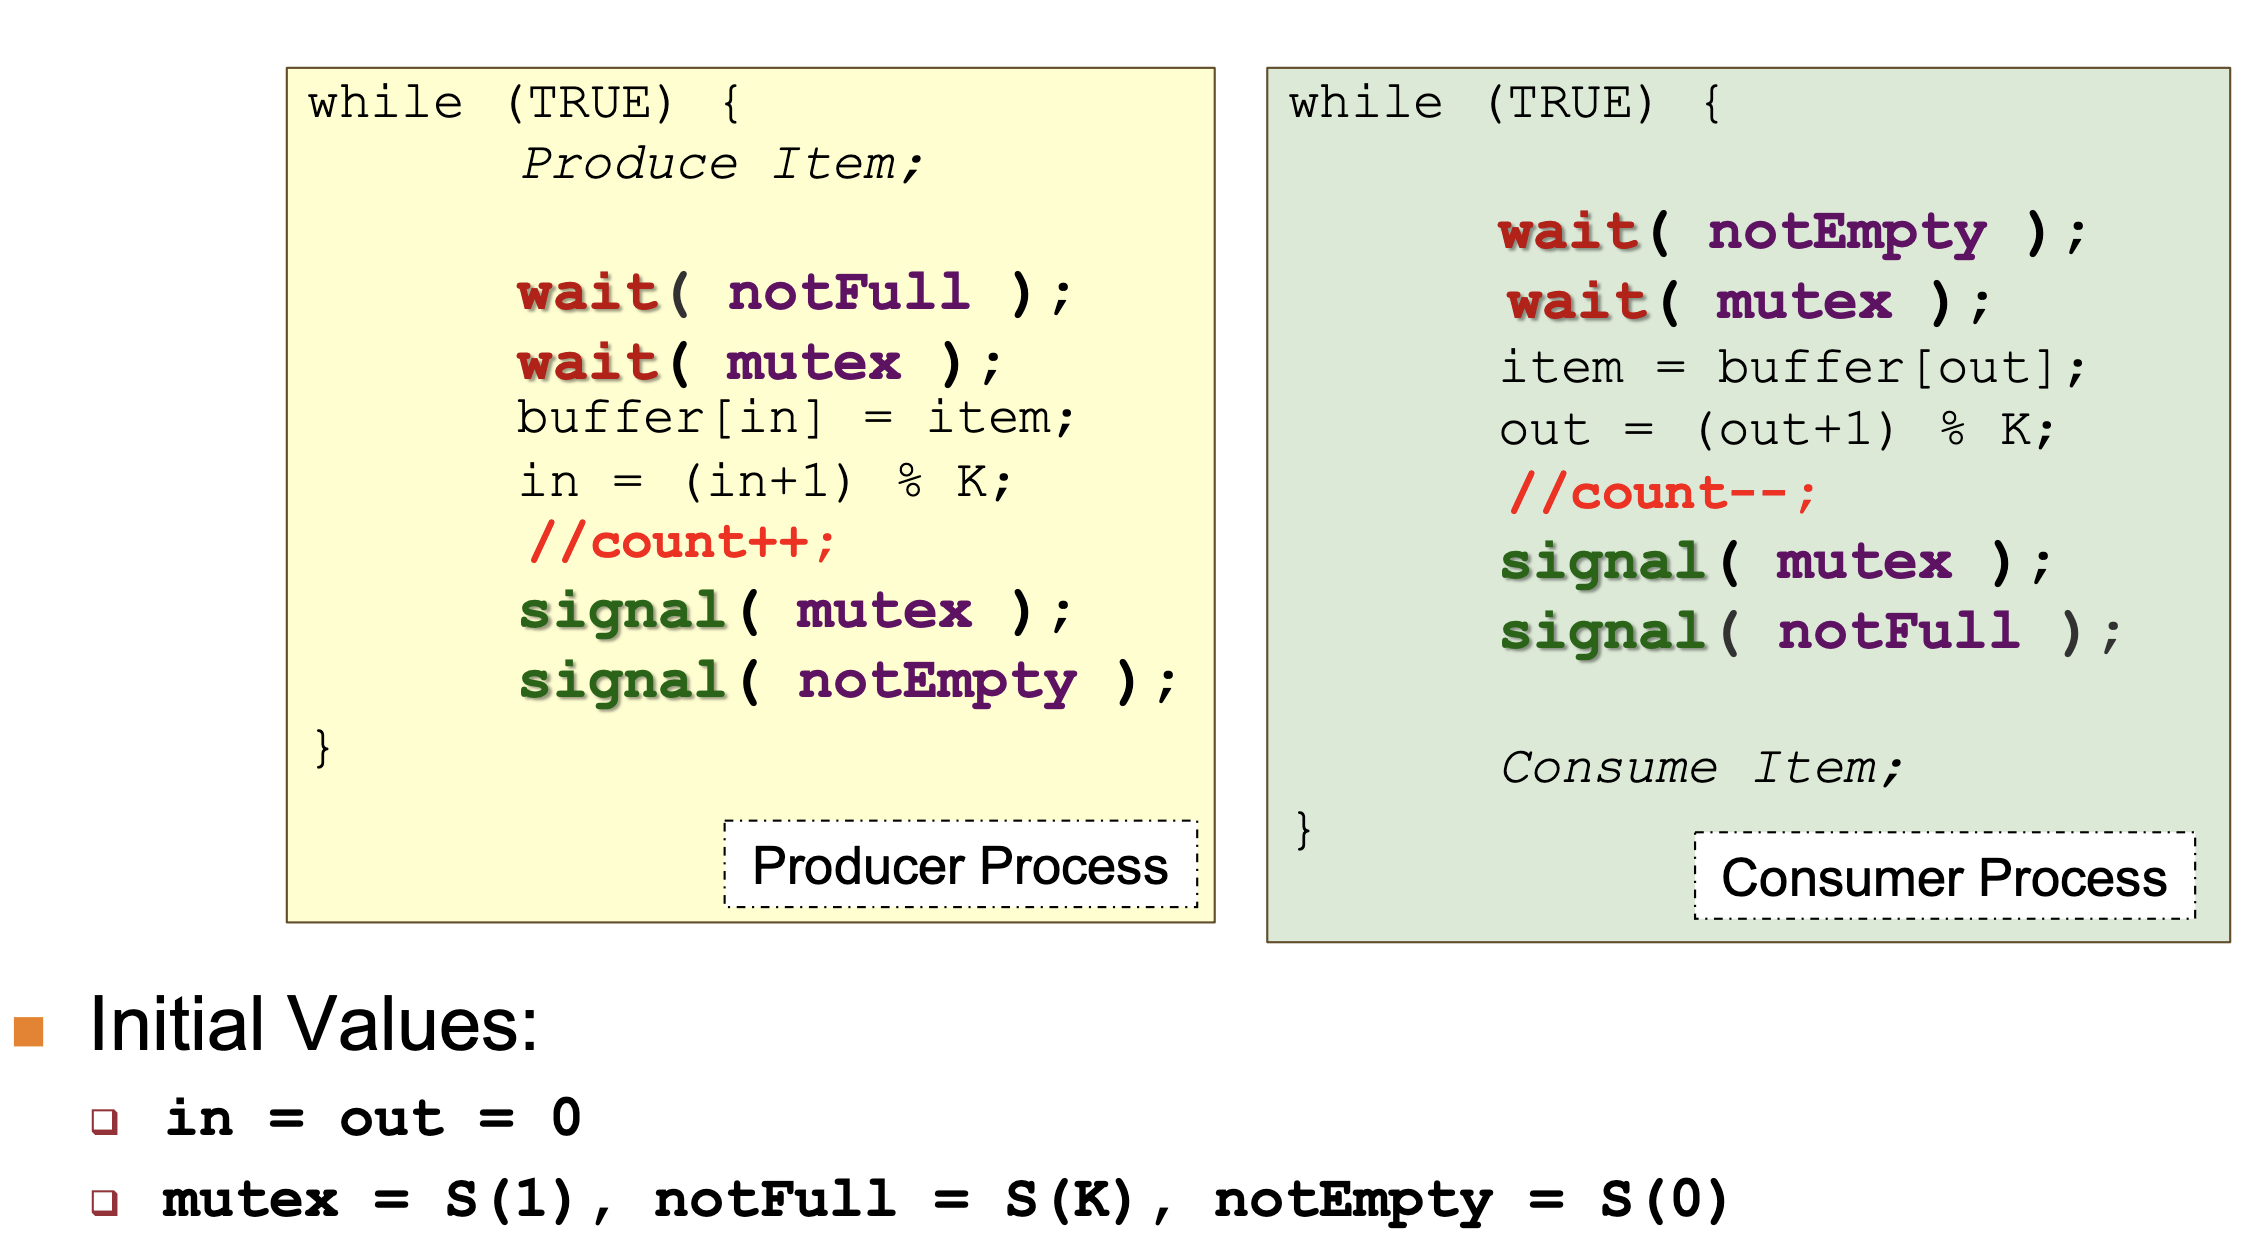
\includegraphics[scale=0.2]{./assets/ProducerConsumer.png}

		Message passing version

		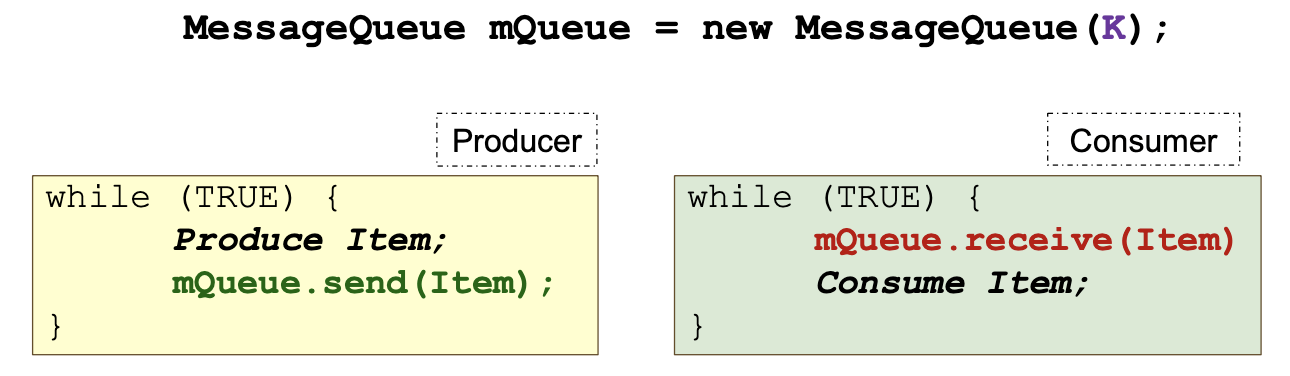
\includegraphics[scale=.34]{./assets/producerConsumerMessage.png}

		Block consumer when buffer empty, block producer when buffer full

		System handles mutual exclusion on buffer operations
		
		\textbf{Reader-Writer (Simple version)}

		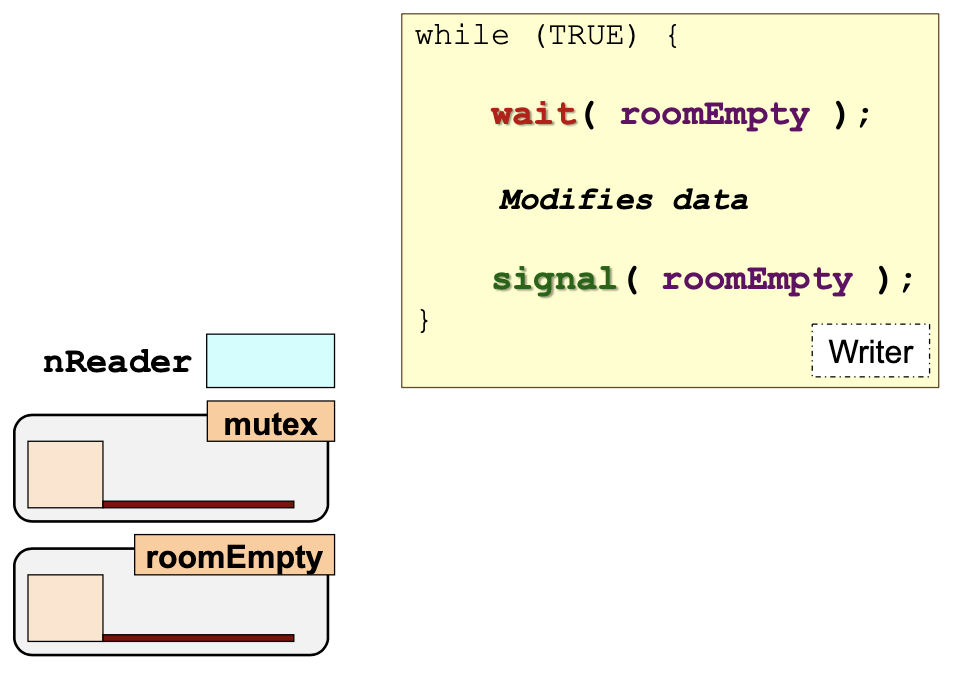
\includegraphics[scale=0.32]{./assets/Writer.png}
		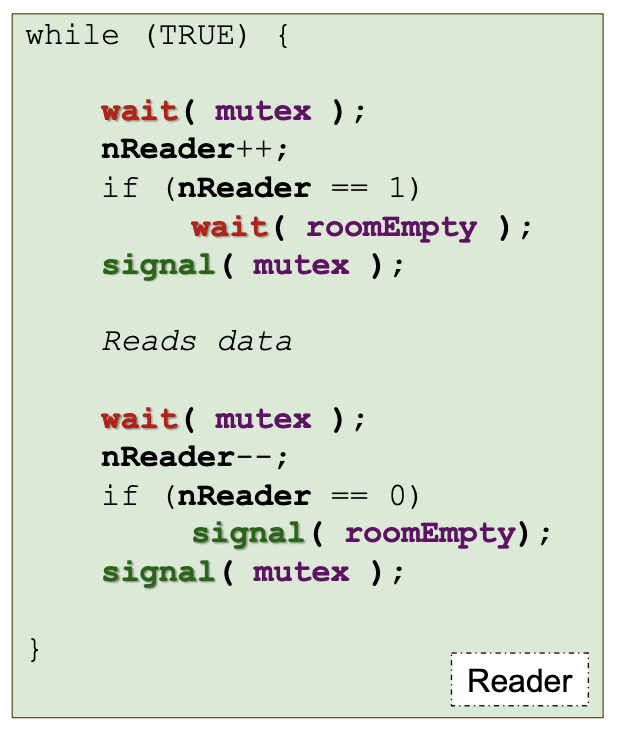
\includegraphics[scale=0.35]{./assets/Reader.png}

		Initial Values: roomEmpty = S(1), mutex = S(1), nReader = 0

		\highlight{Note}: Writers can be \red{starved}

		\textbf{Dining Philosopher}

		1. Limited Seats

		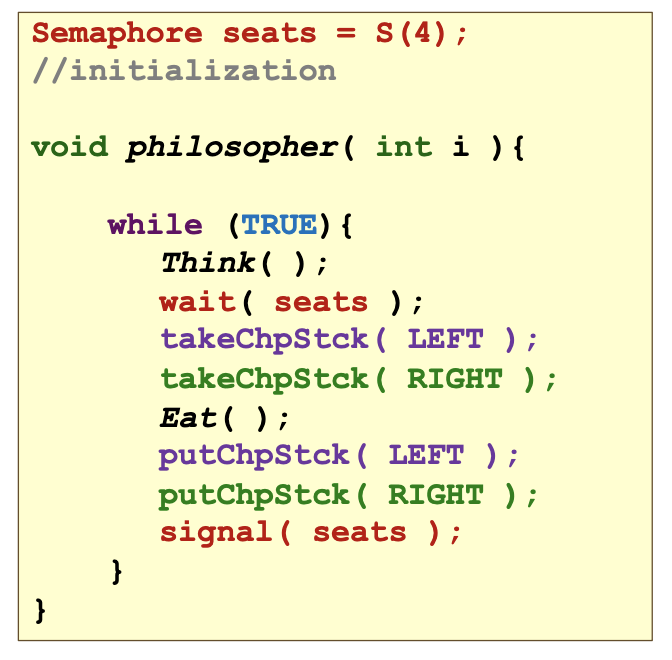
\includegraphics[scale=0.37]{./assets/limitedSeats.png}

		2. Tanenbaum

		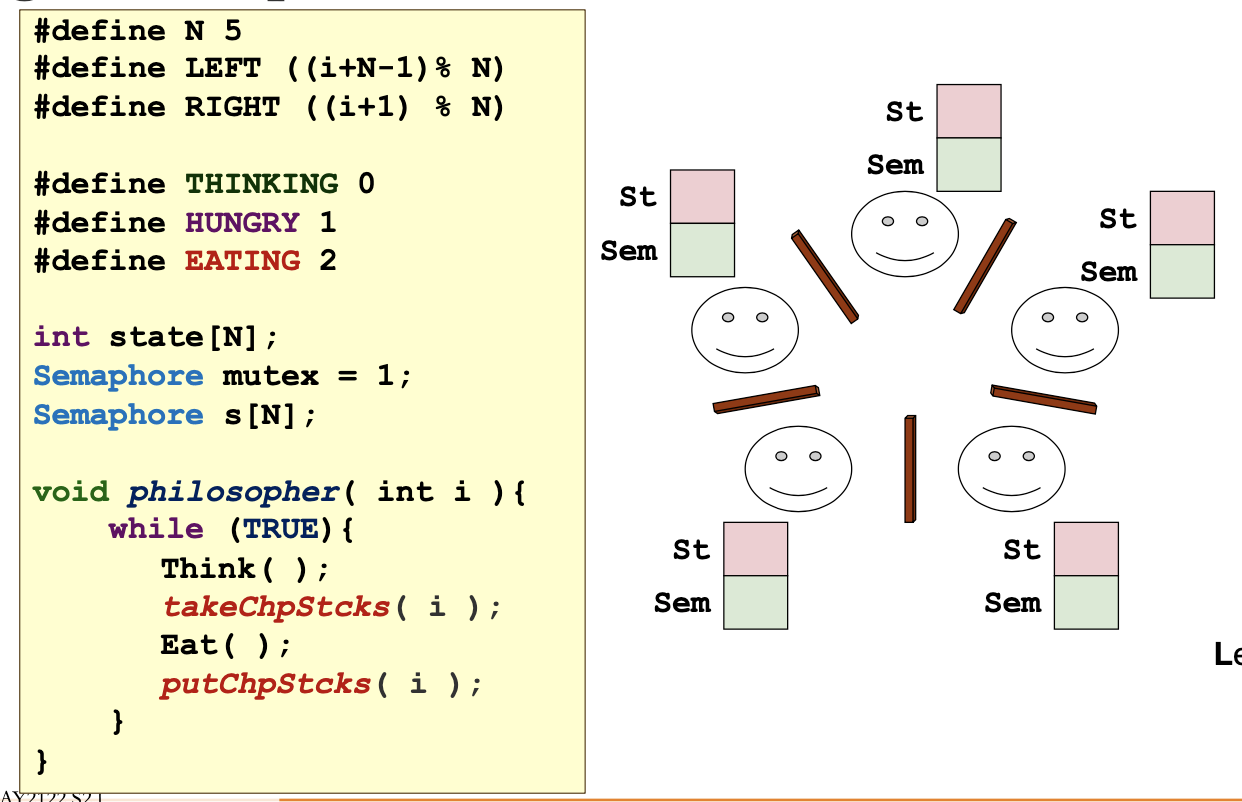
\includegraphics[scale=.38]{./assets/tanenbaum1.png}

		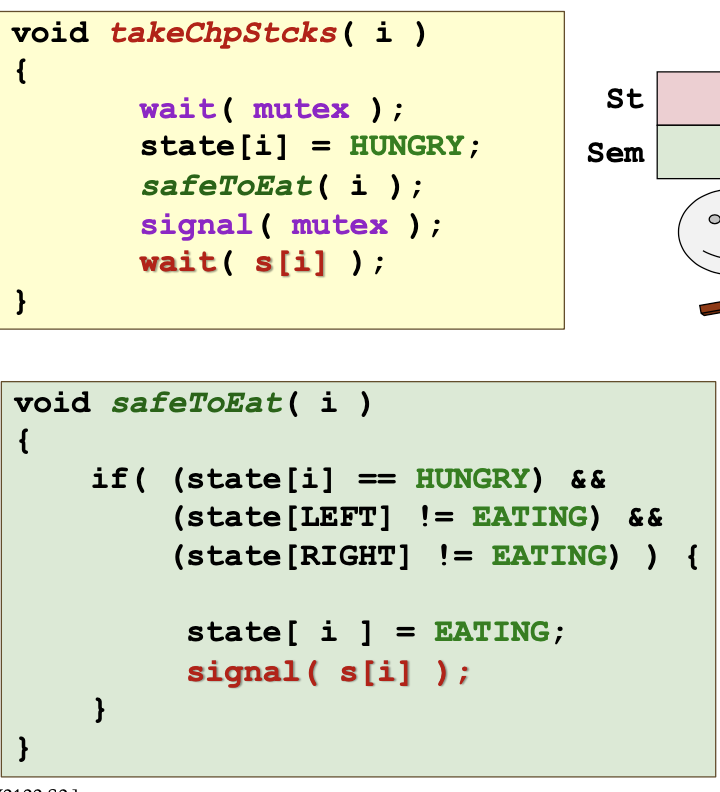
\includegraphics[scale=.38]{./assets/tanenbaum2.png}
		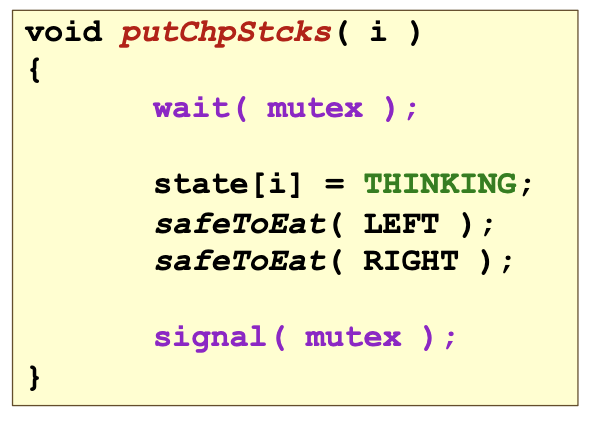
\includegraphics[scale=.38]{./assets/tanenbaum3.png}\\

		\textbf{Layout of Hard Disk}

		\includegraphics*[scale=0.25]{./assets/harddisk}

		\textbf{Pipes and Custom Signal Handler}
		
		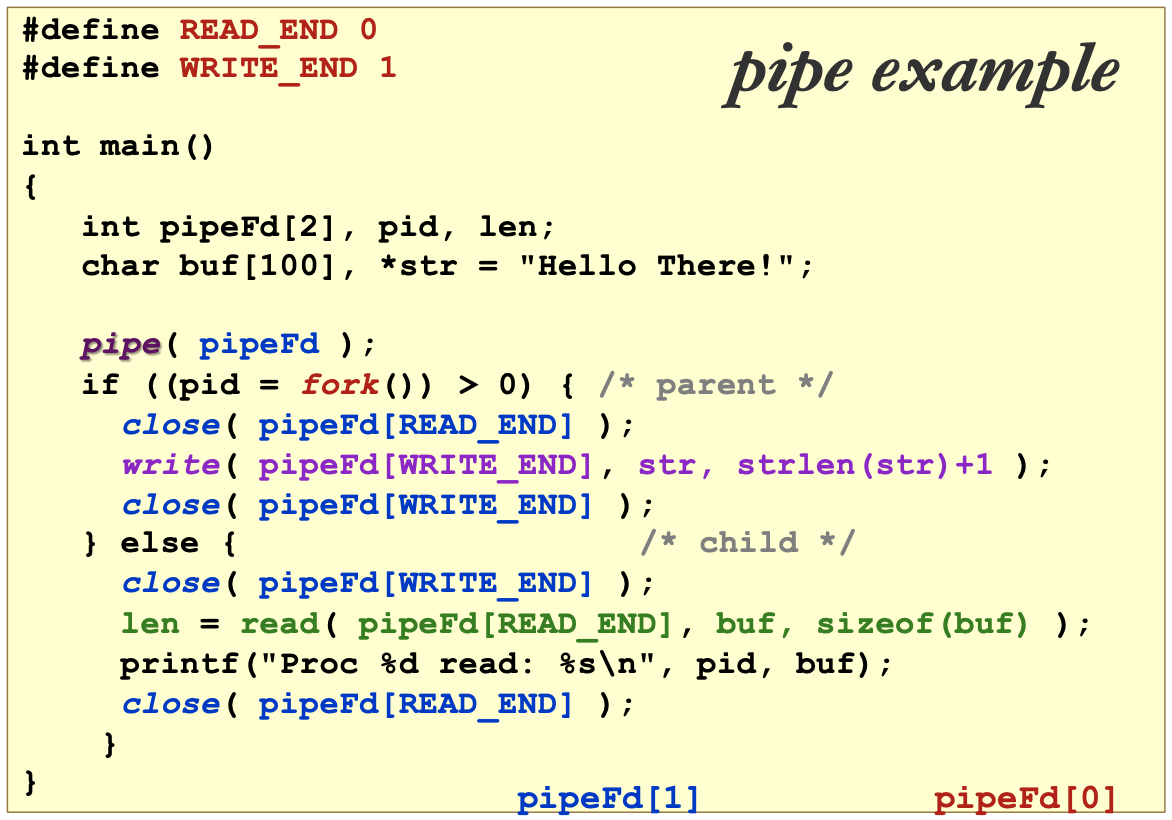
\includegraphics[scale=.37]{./assets/pipe.png}

		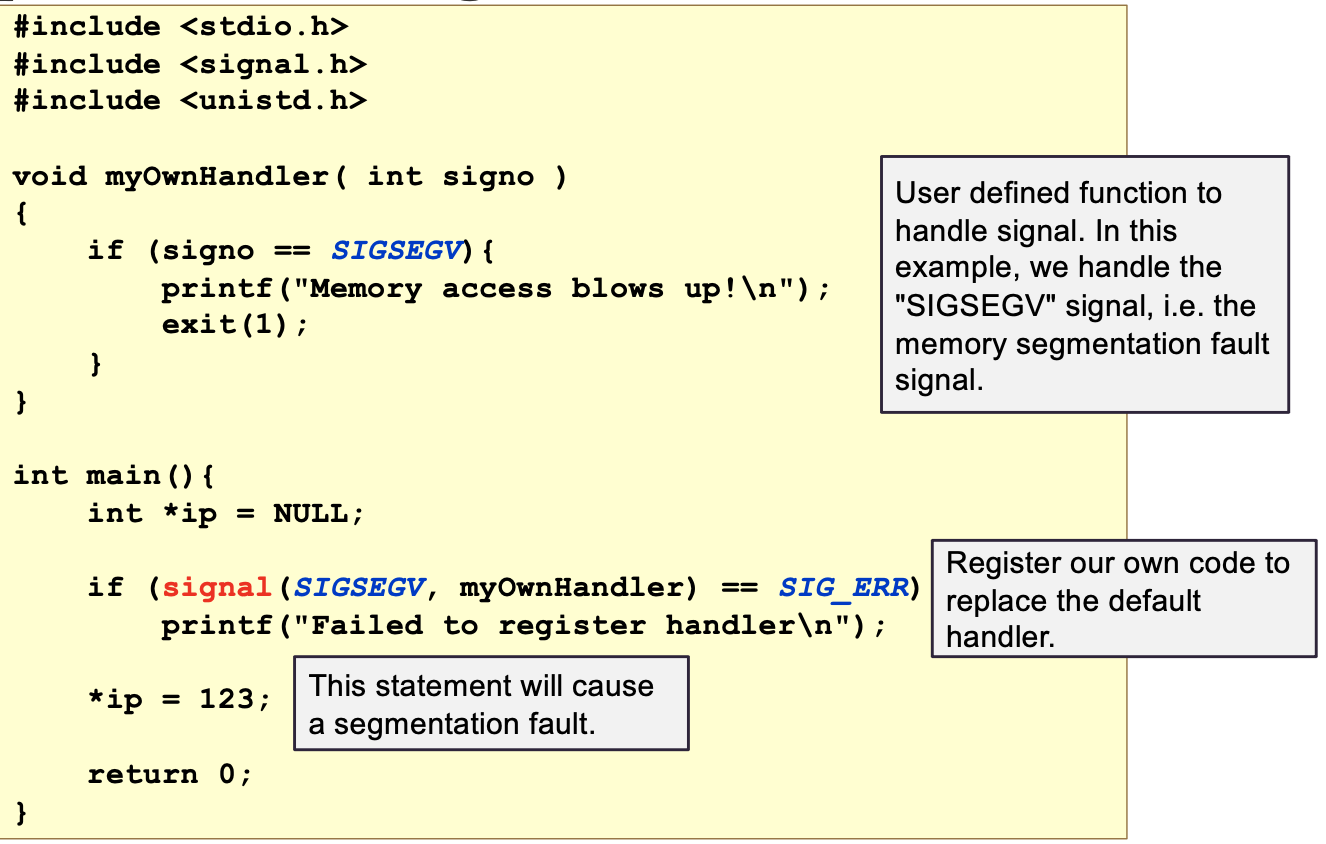
\includegraphics[scale=0.37]{./assets/signalHandler.png}

		\textbf{General Semaphore with mutex}

		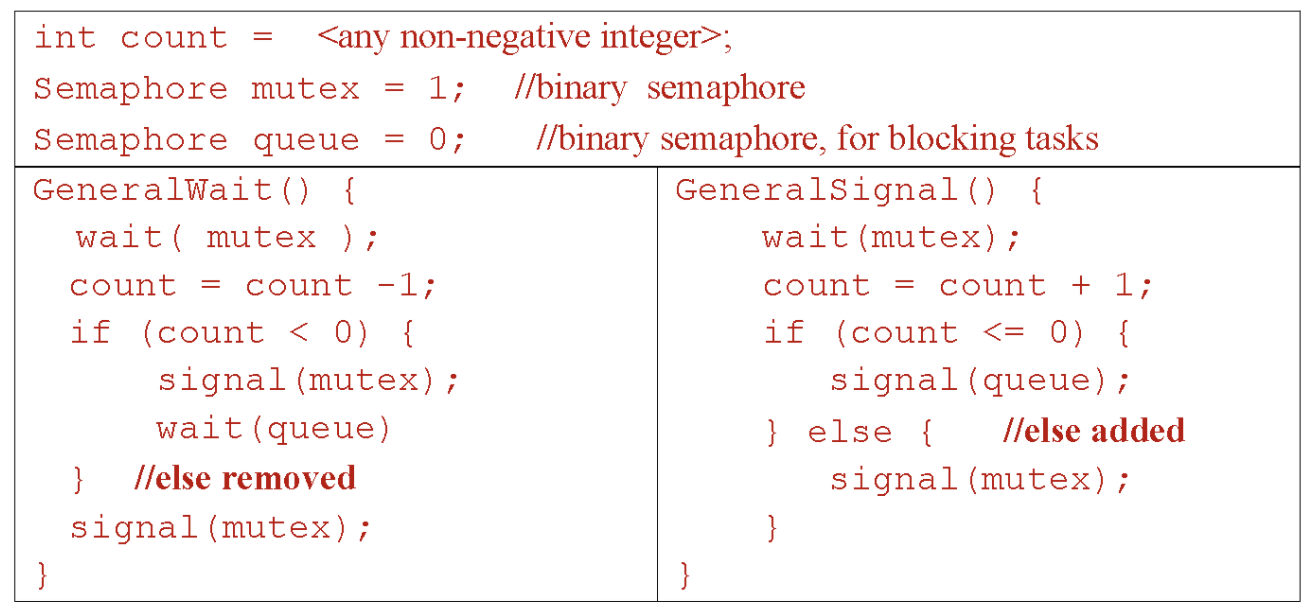
\includegraphics[scale=.4]{./assets/generalSemaphore.png}









		













	  
	\end{multicols*}
\end{document}
